% Selected Supplementary sections for Diffushadow2.
% Evidence audit: manuscript PDFs dated 4 October 2026 and
% Miamm0v0/Diffushadow, commit 9e5edaf707b4c886655205461bb7ab3842c89756.
% Sections S2, S3 and S5 are intentionally outside this draft.
% Current Supplementary Fig. 1--4 numbering is retained provisionally.
% Red TBD markers identify missing or conflicting evidence, not inferred settings.
\documentclass[11pt,a4paper]{article}
\usepackage[margin=25mm]{geometry}
\usepackage[T1]{fontenc}
\usepackage{lmodern}
\usepackage{amsmath,amssymb,bm}
\usepackage{booktabs,longtable,array,tabularx}
\usepackage{xcolor}
\usepackage{graphicx}
\usepackage{caption}
\usepackage{microtype}
\usepackage{enumitem}
\usepackage{multirow}
\usepackage[hidelinks]{hyperref}
\usepackage{fancyhdr}
\usepackage[numbers,sort&compress]{natbib}
\setlength{\parindent}{0pt}
\setlength{\parskip}{0.45em}
\setlength{\emergencystretch}{2em}
\renewcommand{\theequation}{S\arabic{equation}}
\newcommand{\TBD}[1]{\textcolor{red!70!black}{\textsf{[TBD: #1]}}}
\newcommand{\ind}{\mathbf{1}}
\newcommand{\pauli}{\boldsymbol{\sigma}}

\DeclareCaptionLabelSeparator{naturebar}{\space|\space}
\captionsetup{
  font=small,
  labelfont=bf,
  labelsep=naturebar,
  singlelinecheck=false
}
\captionsetup[figure]{name={Supplementary Fig.}}
\captionsetup[table]{name={Supplementary Table}}

% \crefname{figure}{Supplementary Fig.}{Supplementary Figs.}
% \Crefname{figure}{Supplementary Fig.}{Supplementary Figs.}
% \crefname{table}{Supplementary Table}{Supplementary Tables}
% \Crefname{table}{Supplementary Table}{Supplementary Tables}
% \crefname{equation}{Supplementary Eq.}{Supplementary Eqs.}
% \Crefname{equation}{Supplementary Eq.}{Supplementary Eqs.}


\renewcommand{\thesection}{S\arabic{section}}
\newcommand{\sechead}[2]{\section{#2}}
\newcommand{\subhead}[1]{\subsection*{#1}}
\newcolumntype{L}[1]{>{\raggedright\arraybackslash}p{#1}}
\pagestyle{fancy}
\fancyhf{}
\fancyhead[L]{\small Diffushadow }
\fancyhead[R]{\small Supplementary Information}
\fancyfoot[C]{\thepage}
\setlength{\headheight}{14pt}
\begin{document}
\begin{center}
{\LARGE\bfseries Supplementary Information}\par
\vspace{0.5em}
{\large Thermodynamic-limit inference from quantum measurements with discrete diffusion}\par
\vspace{0.5em}

\vspace{0.35em}
% Replace bracketed placeholders; adjust author and affiliation numbers as needed.
% Mark each corresponding author with an asterisk (*).
Yanhong Li\textsuperscript{1},
Mingjun Han\textsuperscript{2},
Ho-Kin Tang\textsuperscript{3,*}\par
\vspace{0.5em}
{\small
\textsuperscript{1}School of Intelligence Science and Engineering, Harbin Institute of Technology, Shenzhen, 518055, China\par
\textsuperscript{2}Université Paris-Saclay, CNRS/IN2P3, IJCLab, Orsay, 91405, France\par
\textsuperscript{3}School of Science, Harbin Institute of Technology, Shenzhen, 518055, China\par
\vspace{0.35em}
\textsuperscript{*}Correspondence to: Ho-Kin Tang
(\href{mailto:denghaojian@hit.edu.cn}{\nolinkurl{denghaojian@hit.edu.cn}}).\par
}
\end{center}

\tableofcontents
\clearpage

\sechead{S1}{Physical models, measurement datasets and numerical references}
\label{supp:models_data}

\subhead{Hamiltonians and operator conventions}
We write $X_i$, $Y_i$ and $Z_i$ for Pauli operators, with eigenvalues $\pm1$,
and $\mathbf{S}_i=\pauli_i/2$ for spin-$1/2$ operators. The one-dimensional
spin models use periodic boundary conditions, so that site labels are interpreted
modulo $N$. The transverse-field Ising (TFI) Hamiltonian is
\begin{equation}
H_{\mathrm{TFI}}(g)=-(1-g)\sum_{i=1}^{N}Z_iZ_{i+1}
                    -g\sum_{i=1}^{N}X_i,
\qquad 0\leq g\leq1.
\label{supp:eq:tfi}
\end{equation}
Thus, $g$ controls both the field and the exchange coefficient; it is not the
field-to-exchange ratio of a Hamiltonian with a fixed exchange coefficient.
The frustrated $J_1$--$J_2$ chain is defined in the Pauli convention as
\begin{equation}
H_{J_1J_2}(\alpha)=J_1\sum_{i=1}^{N}\pauli_i\cdot\pauli_{i+1}
                 +J_2\sum_{i=1}^{N}\pauli_i\cdot\pauli_{i+2},
\qquad J_1=1,\quad \alpha=J_2/J_1.
\label{supp:eq:j1j2}
\end{equation}
In a spin-operator implementation, the corresponding exchange coefficients are
$4J_1$ and $4J_2$, and a reported Pauli spin-dot correlation is four times the
corresponding $\langle\mathbf{S}_i\cdot\mathbf{S}_{i+r}\rangle$.
For the axial next-nearest-neighbour Ising (ANNNI) chain, we use
\begin{equation}
H_{\mathrm{ANNNI}}(g,\kappa)
=-J_1\sum_i Z_iZ_{i+1}+\kappa J_1\sum_i Z_iZ_{i+2}-g\sum_iX_i,
\qquad J_1=1,\quad\kappa=0.4.
\label{supp:eq:annni}
\end{equation}
Here \(g\) denotes the transverse-field coefficient and, unlike Eq.~\ref{supp:eq:tfi}, does not follow the interpolating convention of the TFI model.

The two-dimensional TFI model is defined on a rectangular $L_x\times L_y$
periodic lattice, with $N=L_xL_y$,
\begin{equation}
H_{\mathrm{2D}}(g)=-(1-g)\sum_{\langle\mathbf{r},\mathbf{r}'\rangle}
Z_{\mathbf{r}}Z_{\mathbf{r}'}-g\sum_{\mathbf{r}}X_{\mathbf{r}},
\label{supp:eq:tfi2d}
\end{equation}
where each undirected nearest-neighbour bond is counted once.
For the Rydberg chain, $n_i=|r_i\rangle\langle r_i|=(Z_i+1)/2$ denotes the
excitation occupation. The physical Hamiltonian convention is
\begin{equation}
\frac{H_{\mathrm{Ryd}}}{\Omega}
=\frac12\sum_{i=1}^{N}X_i-d\sum_{i=1}^{N}n_i
+\sum_{r=1}^{R_{\mathrm{cut}}}V_r\sum_{i=1}^{N-r}n_in_{i+r},
\qquad d=\frac{\delta}{\Omega},\quad
V_r=\frac{(R_b/a)^6}{r^6}.
\label{supp:eq:ryd}
\end{equation}
The chain has open ends and $R_b/a=2.35$. 
% The earlier manuscript specifies
% $R_{\mathrm{cut}}=5$. \TBD{RYD-H-EDGE: confirm the interaction cutoff and
% the site-dependent edge terms of the actual open-boundary MPO against
% Eq.~\eqref{supp:eq:ryd}}.

\subhead{Measurement records and dataset partitions}
For the one- and two-dimensional spin models, each record consists of
$\mathbf{P}\in\{X,Y,Z\}^{N}$ and $\mathbf{b}\in\{0,1\}^{N}$. The bases are
sampled independently and uniformly at each site. With $s_i=2b_i-1$, the
reference probability of a complete outcome record is
\begin{equation}
p(\mathbf{b}\mid\mathbf{P},\boldsymbol{\lambda})
=\operatorname{Tr}\!\left[
\rho_{N,\boldsymbol{\lambda}}
\bigotimes_{i=1}^{N}\frac{I+s_iP_i}{2}\right],
\label{supp:eq:measurement_probability}
\end{equation}
where $\rho_{N,\boldsymbol{\lambda}}$ is the numerical ground-state reference.
Sampling uses conditional Born probabilities and state updates, thereby
retaining the joint outcome statistics. These records define local-Pauli
classical shadows~\cite{huang2020predicting}. Rydberg data instead consist of
fixed-$Z$ occupation records $\mathbf{n}\in\{0,1\}^{N}$ sampled from finite
matrix product states (MPS); no random Pauli bases are sampled for this dataset.
The occupation-to-token conversion is specified in Section~\ref{supp:rydberg}.

The initial one-dimensional training sizes are $N\in\{8,10,12,14\}$.
The training grids are
\begin{align}
\mathcal{G}_{\mathrm{TFI}}=\mathcal{G}_{J_1J_2}
 &=\{0,0.25,0.4,0.5,0.6,0.75,0.9,1.0\},\\
\mathcal{G}_{\mathrm{ANNNI}}
 &=\{0,0.25,0.4,0.5,0.6,0.75,0.9,1.0,1.25,1.5,1.75,2.0\}.
\end{align}
These grids refer to $g$, $\alpha$ and $g$, respectively.
Subsequent recursive training uses the retained
exact and previously generated datasets described in main-text Methods. The two-dimensional training set contains the six geometries
$3\times3$, $3\times4$, $3\times5$, $4\times3$, $4\times4$ and $5\times3$.
The same trained two-dimensional model is directly evaluated on $6\times6$
and $7\times7$ lattices. Rydberg training uses $N\in\{16,24,32\}$, with
detunings extending up to $d=5.0$.

The TFI evaluations on thermodynamic-limit inference use 15 uniformly spaced values of $g$ in $[0,1]$. The one-dimensional evaluation grids for the $J_1$--$J_2$ and ANNNI models also contain 15 uniformly spaced values in $[0,1]$
and $[0,2]$, respectively. The evaluation of two-dimensional TFI model is conducted on 8 $g$ values in \{0,0.25,0.4,0.5,0.6,0.75,0.9,1.0\}. The standard one-dimensional generated ensembles contain $M=10{,}000$ records per size and parameter point; the alternative budgets in Section~\ref{supp:decoding_budget} are exceptions. This generated-record count is distinct from the number of records used for training.

% \begin{longtable}{@{}L{0.18\textwidth}L{0.29\textwidth}L{0.45\textwidth}@{}}
% \caption{Dataset inventory. Counts refer to each size and parameter point
% unless otherwise stated.}\label{supp:tab:data_inventory}\\
% \toprule
% Dataset & Sizes and source & Records and partition information \\
% \midrule\endfirsthead
% \toprule Dataset & Sizes and source & Records and partition information \\
% \midrule\endhead
% One-dimensional spin training & $N=8,10,12,14$; ED Pauli records &
% \TBD{TRAIN-COUNTS-1D}; \TBD{SPLIT-1D: training, validation and independent
% test counts, sampling seeds and split rule}. \\
% Recursive spin training & Retained exact records and previous-round
% generated records & Full size, count and checkpoint manifest in Section~S5;
% \TBD{RECURSIVE-MANIFEST}. \\
% Two-dimensional spin training & Six geometries listed above; ED/Lanczos
% Pauli records & \TBD{GRID-2D}; \TBD{TRAIN-COUNTS-2D}; \TBD{SPLIT-2D}. \\
% Two-dimensional evaluation & $6\times6$, $7\times7$; generated Pauli records
% and SSE QMC references & \TBD{EVAL-2D: parameter grid, generated count and
% reference runs}. \\
% Rydberg training & $N=16,24,32$; finite-DMRG/MPS $Z$ records &
% \TBD{RYD-TRAIN-GRID}; \TBD{RYD-TRAIN-COUNTS}; \TBD{RYD-SPLIT}. \\
% Rydberg reconstruction & $N=32$; independently sampled held-out MPS records &
% $1000$ records at $d=0.2,1.8,3.4,5.0$; $500$ records at
% $d=4.0,4.4,4.8,5.2,5.6,6.0$. Shared missing-site masks as in Section~S6. \\
% \bottomrule
% \end{longtable}
% Training, validation and independent test records must be identified at the
% record level. \TBD{DATA-PARTITIONS: identify whether each split uses separate
% measurement draws or a partition of an existing pool; give file identifiers
% and seeds}. \TBD{ED-DEGENERACY: specify ground-state selection and any
% symmetry averaging at degenerate parameter points}.

\subhead{Numerical reference calculations and data generation}

Finite spin systems are treated by exact diagonalization (ED).
For the two-dimensional TFI lattices, the Hamiltonian is represented in matrix-free form and its ground state is obtained using a sparse Lanczos eigensolver with tolerance $10^{-10}$
and a maximum of 10,000 iterations~\cite{lanczos1950iteration}.
The calculation is performed in the full computational basis without
explicit symmetry-sector reduction, using a normalized uniform
positive vector as the initial state. The resulting ground states are
used both to generate projective-measurement records and to evaluate
finite-size observables.

For one-dimensional TFI evaluation, systems with $N\leq10$ are solved
by dense Hermitian diagonalization, whereas larger systems use sparse diagonalization. The
resulting density matrix is symmetrized under the global spin flip,
\begin{equation}
\rho_{\mathrm{sym}}
=
\frac{\rho+P\rho P^\dagger}
{\operatorname{Tr}(\rho+P\rho P^\dagger)},
\qquad
P=X^{\otimes N}.
\end{equation}
This averaging is performed after diagonalization and does not
project the state onto a particular parity sector. No subsequent spin-flip
averaging is applied in this size range. At the exactly degenerate
$g=0$ endpoint, the finite-size $ZZ$ observables considered here are
independent of the choice of state within the ferromagnetic
ground-state manifold.

For finite-size $J_1$--$J_2$ and ANNNI calculations, systems with
$N<12$ are solved by full diagonalization, whereas larger systems are
treated using sparse \texttt{eigsh} with a tolerance of $10^{-10}$.
Parameter sweeps use the converged ground state at the preceding
parameter value as the initial vector for the next calculation. At
the $J_1$--$J_2$ endpoint $J_2=1$, where the lowest levels become
numerically degenerate, twelve low-energy eigenstates are computed.
States within $10^{-8}\max(1,|E_0|)$ of the lowest energy are treated
as the degenerate subspace, and the preceding ground-state vector is
projected onto this subspace and renormalized to define the reference
state. Measurement-data generation uses the same sparse solver; for
the $J_1$--$J_2$ chain, the ground-state branch is followed using
intermediate parameter steps of 0.01. All one-dimensional ED
calculations use the full computational basis without explicit
symmetry-sector reduction.

Thermodynamic-limit references for the frustrated and
competing-interaction chains are obtained using infinite DMRG
(iDMRG)~\cite{mcculloch2008infinite,schollwock2011density}. The calculations
use a two-site unit cell and two-site updates with a mixer, without
conserved spin quantum numbers. The singular-value truncation
threshold is $10^{-12}$, the energy convergence threshold is
$10^{-10}$, and at most 200 sweeps are performed.
The nearest-neighbour $J_1$--$J_2$ reference averages the two bond
parities of the unit cell. ANNNI reference normalization and the
treatment of the disconnected contribution are described in
Section~\ref{supp:shadow_estimators}.
% \TBD{Report the final retained bond dimension(s) and, if needed,
% a brief bond-dimension convergence check.}

For the TFI chain, thermodynamic-limit $ZZ$ correlations are obtained
from the exact free-fermion solution~\cite{pfeuty1970one}, using
the Hamiltonian convention
\begin{equation}
H
=
-(1-g)\sum_i Z_iZ_{i+1}
-g\sum_i X_i .
\end{equation}
The corresponding fermionic contractions are evaluated by adaptive
quadrature over momentum, and correlations at separation $r$ are
computed from the associated $r\times r$ Toeplitz determinant.
The endpoints are evaluated analytically,
\begin{equation}
C_{ZZ}^{\infty}(r,0)=1,
\qquad
C_{ZZ}^{\infty}(r,1)=0
\quad (r>0).
\end{equation}
These values provide the thermodynamic-limit references used in
Fig.~2.

For the $6\times6$ and $7\times7$ two-dimensional TFI tests,
finite-lattice $ZZ$ correlations are evaluated using stochastic
series expansion (SSE) quantum Monte Carlo
(QMC)~\cite{sandvik2003stochastic}. The simulations use the same periodic
torus geometry and Hamiltonian convention as the ED calculations.
Correlations are evaluated for displacements $(0,1)$, $(1,0)$ and
$(0,2)$, corresponding to horizontal nearest neighbours, vertical
nearest neighbours and horizontal separation two, and are averaged
over equivalent lattice pairs. Each parameter point is simulated at
inverse temperature $\beta=128$, using 20,000 thermalization sweeps
followed by 100,000 measurement sweeps grouped into 40 bins. The
reported SSE values are finite-$\beta$ thermal expectation values
and are used as numerical references for the large-lattice tests.

The Rydberg MPS calculations provide projective-measurement records
in the occupation basis and the conditional probabilities entering
the Bayes reference. Their numerical settings and contraction checks
are described in Section~\ref{supp:rydberg}.



\sechead{S2}{Implementation and training configurations}
\label{sec:s2_implementation}

The measurement records described in Section~\ref{supp:models_data} are used to train
separate Diffushadow models for the different Hamiltonians. Here we
describe the token representations, positional encodings, masking
procedure and training configurations underlying the architecture in
main-text Methods, Sections~4.2 and 4.3.

\subhead{Token representations and positional encoding}

For the one-dimensional models, each measurement record is represented
as the interleaved sequence
\[
[\lambda,P_1,b_1,\ldots,P_N,b_N],
\]
where $\lambda$ denotes the Hamiltonian control parameter, $P_i$ the
measurement basis and $b_i$ the corresponding outcome. The control
parameter is mapped to a learned embedding through an affine projection.
Separate embeddings are used for the measurement bases and for the
outcome categories $0$, $1$ and $[\mathrm{MASK}]$, together with
token-type embeddings that distinguish parameter, basis and outcome
tokens. Rotary positional embeddings (RoPE) are applied according to
the interleaved sequence positions, with the parameter token at
position zero and the basis and outcome tokens of site $i$ at positions
$2i-1$ and $2i$, respectively.

The two-dimensional implementation retains the basis and outcome
representations but assigns each site its explicit lattice coordinates.
Tokens are arranged in row-major order, while their spatial positions are specified explicitly by the two-dimensional coordinates. The
control parameter is projected to a vector $c_\lambda$ and added to
the basis and outcome embeddings,
\[
h^{P}_{r,c}
=
e_P(P_{r,c})+e_{\mathrm{type}}(P)+c_\lambda,
\qquad
h^{b}_{r,c}
=
e_b(\widetilde b_{r,c})+e_{\mathrm{type}}(b)+c_\lambda,
\]
where $(r,c)$ denotes the lattice coordinate and $\widetilde b$ is the
partially masked outcome configuration. The basis and outcome tokens
associated with the same site share the same row and column
coordinates.

Spatial information is introduced through axial two-dimensional RoPE.
For each attention head, the query and key representations are divided
between the two lattice axes. The two components are rotated according
to the row and column coordinates and concatenated, for example
\[
\widetilde q_{r,c}
=
\bigl[
R_r q^{\mathrm{row}}_{r,c};
R_c q^{\mathrm{col}}_{r,c}
\bigr],
\]
with the same construction applied to the keys. This provides explicit
two-dimensional positional information independently of the row-major
storage order. A linear output layer applied to the outcome-token
representations predicts the two possible measurement outcomes at each
site.

\subhead{Model architecture}

Diffushadow uses full self-attention Transformer blocks with rotary
positional embeddings, residual connections, layer normalization and
GELU feed-forward networks of width $4d$. The one-dimensional TFI,
$J_1$--$J_2$ and ANNNI models use hidden dimension $d=256$, six
Transformer blocks and eight attention heads. Model-specific
architectural and optimization settings for the reported experiments
are summarized in Table~\ref{tab:s2_training_configurations}.

\subhead{Masking and mixed-size training}

Training follows the masked-outcome objective described in main-text
Methods, Section~4.3. For each record, a masking probability is sampled
and outcome sites are masked independently according to that
probability. Masks are resampled during training, while the Hamiltonian
control parameter and measurement bases remain visible. Cross-entropy
loss is evaluated only on masked outcomes and averaged over the masked
sites in each mini-batch. The masking ranges used for the reported
models are listed in Table~\ref{tab:s2_training_configurations}.

Mixed-size datasets are trained without padding records of different
system sizes into a common sequence length. One-dimensional records are
grouped by system size and two-dimensional records by lattice geometry,
so that each mini-batch contains a common token length and, for the
two-dimensional case, a common lattice shape. Mini-batches from the
different groups are shuffled during each epoch. Batch sizes are
adjusted across system sizes to keep the approximate number of input
tokens per optimization step comparable.

\subhead{Optimization and model selection}

Models are optimized using AdamW. The learning rate, batch size, number
of epochs, learning-rate schedule and positional-scaling settings used
for each experiment are reported in
Table~\ref{tab:s2_training_configurations}. When validation-based model
selection is used, the checkpoint with the lowest masked-outcome
validation loss is retained for evaluation. The recursive training
procedure and the relation between models and generated datasets across
successive rounds are described in main-text Methods, Section~4.5.

\begin{table}[htbp]
\centering
\small
\caption{Training configurations for the reported Diffushadow models.
$d$, $L$ and $H$ denote the hidden dimension, number of Transformer
blocks and number of attention heads, respectively. $\eta$ is the
initial learning rate, $B_{\mathrm{base}}$ is the batch size at the
largest training size and $E$ is the number of training epochs.}
\label{tab:s2_training_configurations}
\begin{tabular}{lccccccccc}
\hline
System
& $d$
& $L$
& $H$
& $\eta$
& $B_{\mathrm{base}}$
& $E$
& $\epsilon$
& \shortstack{LR\\schedule}
& \shortstack{RoPE\\scaling} \\
\hline
1D TFI
& 256 & 6 & 8
& 1e-5
& 128
& 120
& 0.1
& cosine warmup
& 4.0 \\

J$_1$--J$_2$
& 256 & 6 & 8
& 1e-5
& 128
& 120
& 0.1
& cosine warmup
& 4.0 \\

ANNNI
& 256 & 6 & 8
& 1e-5
& 128
& 120
& 0.1
& cosine warmup
& 4.0 \\

2D TFI
& 256
& 6
& 8
& 5e-5
& 128
& 120
& 0.1
& cosine warmup
& 4.0 \\

Rydberg
& 128
& 4
& 8
& 1e-5
& 128
& 100
& 0.1
& cosine warmup
& 4.0 \\
\hline
\end{tabular}
\end{table}



\sechead{S3}{Classical-shadow observable estimators}
\label{supp:shadow_estimators}

\subhead{Inverse-channel estimators and aggregation}
For a uniformly sampled local-Pauli record
$(\mathbf{P}_t,\mathbf{b}_t)$, let $s_{t,i}=2b_{t,i}-1$.
The inverse-channel snapshot and its single-site Pauli estimator
are~\cite{huang2020predicting}
\begin{equation}
\widehat{\rho}_t
=
\bigotimes_{i=1}^{N}
\left(3\frac{I+s_{t,i}P_{t,i}}{2}-I\right),
\qquad
\widehat{\sigma}^{\alpha}_{t,i}
=
3s_{t,i}\ind[P_{t,i}=\alpha].
\label{supp:eq:local_shadow}
\end{equation}
For a Pauli string $W=\bigotimes_iW_i$ with support
$\mathcal{I}=\{i:W_i\ne I\}$, its single-record estimator is
\begin{equation}
\widehat{W}_t
=
\operatorname{Tr}(W\widehat{\rho}_t)
=
\prod_{i\in\mathcal{I}}
3s_{t,i}\ind[P_{t,i}=W_i].
\label{supp:eq:pauli_string}
\end{equation}
Identity factors equal one. Products involving the same site are
first reduced using the Pauli algebra; in particular, $Z_i^2=I$
is estimated as one.

Spatial averaging is performed within each record. For a translated
observable, denote the resulting per-record value by $u_t$.
The records are divided into $K=10$ equal consecutive groups
$\mathcal{B}_k$, and median-of-means aggregation gives
\begin{equation}
\overline{u}_k
=
\frac{1}{|\mathcal{B}_k|}
\sum_{t\in\mathcal{B}_k}u_t,
\qquad
\widehat{u}_{\mathrm{MoM}}
=
\operatorname{median}_{k=1,\ldots,K}\overline{u}_k.
\label{supp:eq:mom}
\end{equation}
All record budgets reported here are divisible by $K$.
For even \(K\), we use the lower of the two central group means; for \(K=10\), this corresponds to the fifth ordered group mean.
% \TBD{MOM-2D: median convention used in the final two-dimensional
% evaluation}.
The same estimators are applied to exact and generated measurement
ensembles. Direct ED or MPS expectation values are evaluated from
the reference states. Snapshot bootstrap resampling is performed on whole records, retaining each record's basis and outcome sequences together.

\subhead{Spin correlations and two-dimensional displacements}
For a periodic chain and nonzero separation $r$, define the group estimate
\begin{equation}
\widehat{C}^{(k)}_{\alpha\alpha,N}(r)
=\frac{1}{|\mathcal{B}_k|N}
\sum_{t\in\mathcal{B}_k}\sum_{i=1}^{N}
\widehat{\sigma}^{\alpha}_{t,i}
\widehat{\sigma}^{\alpha}_{t,i+r}.
\label{supp:eq:component_correlation}
\end{equation}
The reported TFI $ZZ$ correlation is the MoM of these group estimates
for $\alpha=Z$. It is the unconnected correlation
$N^{-1}\sum_i\langle Z_iZ_{i+r}\rangle$, with no subtraction of
single-site magnetizations. The $J_1$--$J_2$ spin-dot estimate is
\begin{equation}
\widehat{C}_{\mathrm{spin},N}(r)
=\sum_{\alpha=X,Y,Z}
\operatorname{median}_{k}\widehat{C}^{(k)}_{\alpha\alpha,N}(r).
\label{supp:eq:spin_dot}
\end{equation}
Thus, each spin component is therefore aggregated before summation over components, rather than applying the median after the component sum.

On the two-dimensional torus, the analogous per-record estimator is
\begin{equation}
u_t(\boldsymbol{\Delta})=
\frac{1}{L_xL_y}\sum_{x=0}^{L_x-1}\sum_{y=0}^{L_y-1}
\widehat{Z}_{t,(x,y)}
\widehat{Z}_{t,(x+\Delta_x,y+\Delta_y)},
\label{supp:eq:2d_correlation}
\end{equation}
where both coordinates are periodic. The three reported displacements
are $(0,1)$, $(1,0)$ and $(0,2)$: nearest neighbours in the two lattice
directions and separation two along the second coordinate.
The generated records and SSE reference use these same spatial averages.
% \TBD{2D-AXIS-LABELS: match coordinate names to the final figure labels}.

\subhead{ANNNI structure factors}
The finite-size longitudinal structure factor is
\begin{equation}
S_{Z,N}(q)=\frac1N\sum_{i,j=1}^{N}
\cos[q(i-j)]\langle Z_iZ_j\rangle
=\sum_{r=0}^{N-1}\cos(qr)C_{ZZ,N}(r),
\label{supp:eq:annni_sf}
\end{equation}
for the commensurate momenta used here, $q=\pi$ and $q=\pi/2$.
The reported $q=\pi/2$ comparisons use sizes divisible by four.
There is no further division by $N$. The self-correlation is
$C_{ZZ,N}(0)=1$. In the measurement estimator, the Fourier sum is formed
\emph{inside each group} before MoM aggregation:
\begin{equation}
\widehat{S}^{(k)}_{Z,N}(q)
=1+\sum_{r=1}^{N-1}\cos(qr)\widehat{C}^{(k)}_{ZZ,N}(r),
\qquad
\widehat{S}_{Z,N}(q)=\operatorname{median}_k
\widehat{S}^{(k)}_{Z,N}(q).
\label{supp:eq:annni_sf_estimator}
\end{equation}
This procedure is not a Fourier sum of separately aggregated correlations.
The finite-size observable contains the full, unconnected correlation.
For a translation-invariant state and the nonzero commensurate momenta
above, the uniform disconnected contribution vanishes exactly.

The infinite-MPS reference is evaluated from connected correlations
$C^c(r)=\langle Z_0Z_r\rangle-\langle Z_0\rangle\langle Z_r\rangle$.
The infinite-MPS reference uses a one-sided correlation sum truncated at \(r=199\). For comparison with the two-sided convention used in the figures, we evaluate
\begin{equation}
S^{\mathrm{ref}}_Z(q)
=C^c(0)+2\sum_{r=1}^{199}\cos(qr)C^c(r)
=2S^{\mathrm{stored}}_Z(q)-C^c(0).
\label{supp:eq:sf_reference}
\end{equation}
where $C^c(0)=1-m_z^2$.
% \TBD{ANNNI-REF-CHECK: confirm the reference files, unit-cell magnetization
% convention and convergence with the correlation cutoff}. This comparison
% requires the disconnected term and normalization to describe the same
% observable in the finite and infinite systems.

\subhead{$X$ strings and energy}
The $X$-string observable of length $\ell$ is the translated product
\begin{equation}
X_{\ell,N}=\frac1N\sum_{i=1}^{N}
\left\langle\prod_{a=0}^{\ell-1}X_{i+a}\right\rangle,
\quad
\widehat{X}^{(k)}_{\ell,N}
=\frac{1}{|\mathcal{B}_k|N}
\sum_{t\in\mathcal{B}_k}\sum_i
\prod_{a=0}^{\ell-1}\widehat{X}_{t,i+a}.
\label{supp:eq:x_string}
\end{equation}
The estimate is $\operatorname{median}_k\widehat{X}^{(k)}_{\ell,N}$.
Supplementary Fig.~1 evaluates $\ell=1,\ldots,5$, while the decoding
comparison uses $\ell=1,3,5$. These are unconnected Pauli-string
expectations, without an additional order-parameter rescaling.

For the TFI model, the total energy estimate is constructed by summing
the Hamiltonian terms within each group:
\begin{equation}
\widehat{E}^{(k)}_{\mathrm{TFI}}
=-\frac{1}{|\mathcal{B}_k|}\sum_{t\in\mathcal{B}_k}\sum_i
\left[(1-g)\widehat{Z}_{t,i}\widehat{Z}_{t,i+1}
+g\widehat{X}_{t,i}\right],
\qquad
\widehat{E}_{\mathrm{TFI}}=\operatorname{median}_k
\widehat{E}^{(k)}_{\mathrm{TFI}}.
\label{supp:eq:tfi_energy}
\end{equation}
The energy density is $\widehat{e}=\widehat{E}/N$. The same within-group Hamiltonian sum is used if $J_1$--$J_2$ or ANNNI
energies are evaluated: the group-level spin-dot correlations or $ZZ$
correlations and $X$ mean are combined with the coefficients in
Eqs.~\eqref{supp:eq:j1j2} and \eqref{supp:eq:annni}, multiplied by $N$,
and then aggregated. Energy is not reconstructed by combining separately
reported MoM observables.

\sechead{S4}{Rydberg reconstruction and MPS conditional calculations}
\label{supp:rydberg}

\subhead{Encoding, reference states and held-out records}
Rydberg measurement records contain occupations $n_i\in\{0,1\}$,
where $n_i=1$ denotes an excitation. In the MPS representation,
physical index $b_i^{\mathrm{MPS}}=0$ corresponds to an occupied site
and $b_i^{\mathrm{MPS}}=1$ to an empty site. Occupations are therefore
obtained as $n_i=1-b_i^{\mathrm{MPS}}$ before evaluating physical
observables. All measurement-basis tokens supplied to Diffushadow
are fixed to $Z$. The eigenvalue convention in Section~\ref{supp:shadow_estimators} applies
to local-Pauli records; Rydberg statistics are evaluated directly
from the occupations $n_i$.

Reference states are obtained by finite open-chain DMRG, and
measurement records are sampled from their MPS Born
distributions~\cite{schollwock2011density,ferris2012perfect}.
Ground-state calculations use two-site updates with a mixer,
a singular-value threshold of $10^{-10}$, an energy convergence
threshold of $10^{-9}$ and at most 40 sweeps.
% \TBD{RYD-MPS-RUNS: bond-dimension limits and attained dimensions,
% initial states, convergence checks and software versions}.
The finite-chain Hamiltonian and boundary conventions for both
data generation and conditional-reference calculations are specified
in Section~\ref{supp:models_data}. 
% \TBD{RYD-H-EDGE}.

Reconstruction is evaluated on independently sampled held-out
records at $N=32$. The initial evaluation grid contains $M_d=1000$
records at each $d\in\{0.2,1.8,3.4,5.0\}$, generated with sampling
seed 4242. The extended grid contains $M_d=500$ records at each
$d\in\{4.0,4.4,4.8,5.2,5.6,6.0\}$.
% \TBD{RYD-EXT-SEEDS: sampling seeds for the extended grid}.
% The trained checkpoint
% \texttt{ryd\_rb2.35\_oseq\_final.pth} is applied directly to
% reconstruction without additional task-specific training.

For each record $s$, the missing-site set $\mathcal{M}_s$ is sampled
uniformly without replacement from all subsets containing
$k=\max\{1,\operatorname{round}(fN)\}$ sites. Its complement
$\mathcal{O}_s$ contains the observed sites. At $N=32$, the nominal
loss setting $f=0.3$ gives exactly $k=10$ missing sites per record.
Conditional sampling, deterministic decoding, unconditioned fill
and the Bayes calculation use the same intact records and
per-record missing-site masks.
% \TBD{RYD-MASK-SEEDS: per-detuning mask seeds or their derivation}.

\subhead{Conditional completion and controls}
For each record $s$, only outcome tokens at sites in
$\mathcal{M}_s$ are initialized to \texttt{[MASK]}. At each update,
Diffushadow predicts the outcome distributions at all remaining
missing sites, selects the site with the lowest predictive entropy,
and fills its outcome token. Observed outcomes and previously
completed tokens remain fixed. The updated record is then evaluated
again, giving exactly $k$ updates for a record with $k$ missing sites.

For ensemble reconstruction, the selected outcome is sampled from
the predicted distribution at temperature $\tau=1$, with one
completion per intact record. For missing-site accuracy, the selected
outcome is assigned by stepwise argmax. The unconditioned-fill control
generates a complete configuration conditioned on $d$ and the fixed
measurement basis alone. Its occupations are inserted at
$\mathcal{M}_s$, while the original observed occupations are retained.
For the site-density accuracy baseline, the reference MPS marginal
$\rho_j(d)=\langle n_j\rangle$ gives the prediction
$\ind[\rho_j(d)>1/2]$ at each missing site. The unconditioned-fill
control evaluates the contribution of record-specific conditioning
to ensemble reconstruction, whereas the site-density baseline
evaluates its contribution to missing-site prediction.

For an ensemble of $M_d$ records, we define
$\widehat{\rho}_i=M_d^{-1}\sum_s n_i^{(s)}$ and
$\widehat{G}_{ij}=M_d^{-1}\sum_s n_i^{(s)}n_j^{(s)}$.
The connected density structure factor is
\begin{equation}
\widehat{S}(q)
=
\frac{1}{N}\sum_{i,j=1}^{N}\cos[q(i-j)]
\left(
\widehat{G}_{ij}-\widehat{\rho}_i\widehat{\rho}_j
\right).
\label{supp:eq:ryd_sf}
\end{equation}
The sum uses open-chain site coordinates and includes the diagonal
contribution $\widehat{\rho}_i(1-\widehat{\rho}_i)$.
The covariance is evaluated with the $1/M_d$ ensemble normalization.
Structure factors are evaluated on the grid
$q_m=m\pi/60$, $m=0,\ldots,60$, which includes $q=2\pi/3$.
The same grid is used for the MPS reference and reconstructed ensembles.


\subhead{Conditional marginals from the reference MPS}
For the observed occupations in record $s$, define the projector
\begin{equation}
\Pi_s
=
\prod_{i\in\mathcal{O}_s}
|n_i^{(s)}\rangle\langle n_i^{(s)}|.
\end{equation}
The reference conditional excitation probability at a missing site is
\begin{equation}
p_{s,j}
=
\frac{
\langle\psi_d|\Pi_s n_j\Pi_s|\psi_d\rangle
}{
\langle\psi_d|\Pi_s|\psi_d\rangle
},
\qquad j\in\mathcal{M}_s.
\label{supp:eq:ryd_conditional}
\end{equation}
The denominator is the probability of the observed pattern after
summing over all missing occupations. The reference conditions only
on the original observed outcomes; occupations generated during
completion are not included in $\Pi_s$.

We evaluate these marginals by contracting the open-chain MPS in
a double-layer representation. Let $A_i^\nu$ denote its local
tensors, with physical index $\nu=0$ corresponding to an occupied
site and $\nu=1$ to an empty site. For each record, define
\begin{equation}
w_{s,i}(\nu)
=
\begin{cases}
\ind[\nu=1-n_i^{(s)}], & i\in\mathcal{O}_s,\\
1, & i\in\mathcal{M}_s.
\end{cases}
\label{supp:eq:mps_allowed}
\end{equation}
The physical index is therefore fixed at observed sites and summed
over at missing sites. Starting from a scalar open-boundary
environment, the left contraction obeys
\begin{equation}
L_{s,i+1}(c,d)
=
\sum_{a,b,\nu}
L_{s,i}(a,b)\,w_{s,i}(\nu)
(A_i^\nu)_{ac}(A_i^\nu)_{bd}^{*}.
\label{supp:eq:mps_left}
\end{equation}
Right environments are contracted analogously from the opposite end.
If $L_{s,j}$ and $R_{s,j}$ exclude site $j$, its two unnormalized
weights are
\begin{equation}
Q_{s,j}(\nu)
=
\sum_{a,b,c,d}
L_{s,j}(a,b)
(A_j^\nu)_{ac}(A_j^\nu)_{bd}^{*}
R_{s,j}(c,d),
\qquad
p_{s,j}
=
\frac{Q_{s,j}(0)}
{Q_{s,j}(0)+Q_{s,j}(1)}.
\label{supp:eq:mps_probability}
\end{equation}
Reference MPSs are brought to canonical form
before contraction. The reference MPSs have maximum bond dimensions ranging from 26 to 100, with a singular-value cutoff of $10^{-10}$ for SVD
truncation. The resulting conditional probabilities are those of the numerical reference MPS.

The expected Bayes-optimal missing-site accuracy is
\begin{equation}
A_{\mathrm{Bayes}}(d)
=
\frac{1}{M_d k}
\sum_{s=1}^{M_d}\sum_{j\in\mathcal{M}_s}
\max\{p_{s,j},1-p_{s,j}\}.
\label{supp:eq:bayes}
\end{equation}
This quantity maximizes the expected number of correct individual
site predictions under the observed information. It does not require
identifying the most probable joint configuration of all missing
sites. Model accuracy is measured against the withheld occupations
in the intact records, whereas Eq.~\eqref{supp:eq:bayes} gives an
expected accuracy. Finite-sample model accuracies may therefore lie
slightly above the reference expectation.

As a numerical check, conditional marginals with no observed sites
are compared with the density profile obtained directly from DMRG.
The maximum absolute discrepancy in the reported reference
calculations is of order $10^{-16}$. Calculations were retained only when this discrepancy was below $5\times10^{-3}$.
For numerical evaluation of Eq.~\eqref{supp:eq:mps_probability},
the real parts of the contracted weights are normalized by their
sum, without denominator regularization or probability clipping.

\subhead{Blockade and multisite diagnostics}
For each record $s$, let $\mathcal{M}_s$ denote the set of missing
sites. A nearest-neighbour pair crosses the observed/reconstructed
boundary when exactly one of its sites belongs to $\mathcal{M}_s$.
We therefore define
$a_{s,i}=|\ind[i\in\mathcal{M}_s]-\ind[i+1\in\mathcal{M}_s]|$.
For $M_d$ records at detuning $d$, the boundary blockade-violation
rate is
\begin{equation}
V_{\mathrm{boundary}}
=
\frac{
\sum_{s=1}^{M_d}\sum_{i=1}^{N-1}
a_{s,i}n_i^{(s)}n_{i+1}^{(s)}
}{
\sum_{s=1}^{M_d}\sum_{i=1}^{N-1}a_{s,i}
}.
\label{supp:eq:blockade}
\end{equation}
The site sum follows the open-chain geometry. The denominator counts
all scored boundary pairs across records, and the numerator counts
those in which both sites are excited. The same missing-site masks
define the scored pairs for intact records, conditional completion
and unconditioned fill. Reported percentages are
$100V_{\mathrm{boundary}}$.

To assess multisite statistics, we evaluate period-three occupation
products at orders $\ell=2$ and $\ell=8$. Their spatially averaged
correlator is
\begin{equation}
G_\ell
=
\frac{1}{N-3(\ell-1)}
\sum_{i=1}^{N-3(\ell-1)}
\left\langle
\prod_{m=0}^{\ell-1}n_{i+3m}
\right\rangle,
\label{supp:eq:ryd_multisite}
\end{equation}
where the brackets denote an average over all $M_d$ records for the
intact, conditionally completed and unconditioned-fill ensembles.
Only origins for which every site in the product lies within the
open chain are included.

For the complete-case estimator, define
$J_{s,i,\ell}=\prod_{m=0}^{\ell-1}
\ind[i+3m\notin\mathcal{M}_s]$.
At each origin $i$, the occupation product is averaged over records
with $J_{s,i,\ell}=1$, and the resulting origin-wise means are then
averaged spatially. Origins with no usable records are assigned
undefined means and omitted from this correlator average. The mean
number of usable records is
\begin{equation}
\overline{M}_{\mathrm{usable},\ell}
=
\frac{1}{N-3(\ell-1)}
\sum_{i=1}^{N-3(\ell-1)}
\sum_{s=1}^{M_d}J_{s,i,\ell}.
\label{supp:eq:usable}
\end{equation}
This count is averaged over all valid origins, including any with
zero usable records. A record may contribute at one origin and be
excluded at another. When $k$ missing sites are selected uniformly
without replacement from $N$ sites, the probability that a specified
$\ell$-site set remains fully observed is
$\binom{N-\ell}{k}/\binom{N}{k}$.
% \TBD{RYD-COMPLETE-CASE: confirm the empty-origin handling and the
% uncertainty calculation for the spatially averaged estimates}.

\sechead{S5}{Attention analysis and causal-mask control}
\label{supp:attention}

\subhead{Analysis inputs and attention-weighted distance}
The analysis in Fig.~2e--g uses a fixed TFI checkpoint in evaluation mode,
with all outcome tokens set to \texttt{[MASK]}. Basis tokens are sampled
independently and uniformly from $X,Y,Z$ at every site, and the same
basis configurations are reused across the scanned values of $g$ at a
given $N$. No generated outcomes are inserted during this attention
measurement. 
% \TBD{ATTN-CKPT: checkpoint and training-size set};
% \TBD{ATTN-INPUTS: numbers of configurations, seeds, $N$ and $g$ grids}.

Let $A^{(\ell,h)}_{qk}$ be the post-softmax attention weight from query
token $q$ to key token $k$ in layer $\ell$ and head $h$. Masked outcome
tokens are the queries. Both $P_i$ and $b_i$ have site label $i$;
the parameter token has no site label. For
$\mathcal{S}=\{P_i,b_i\}_{i=1}^{N}$ and
$d_N(i,j)=\min\{|i-j|,N-|i-j|\}$, define
\begin{equation}
D^{(\ell,h)}(q)=
\frac{\sum_{k\in\mathcal{S}}A^{(\ell,h)}_{qk}
d_N(s(q),s(k))}
{\lfloor N/2\rfloor\sum_{k\in\mathcal{S}}A^{(\ell,h)}_{qk}}.
\label{supp:eq:attention_distance}
\end{equation}
The denominator conditions the spatial measure on attention assigned to
basis and outcome keys and normalizes the maximum periodic distance to
one. Same-site basis and outcome keys are included with zero distance;
the parameter key is excluded. The query-wise ratios are averaged over
query sites and basis configurations, then over all heads and layers for
Fig.~2e. Ratios are not formed after pooling attention rows.

\subhead{Site kernels and physical-correlation comparison}
The signed displacement $\delta_N(i,j)$ is obtained from $(j-i)\bmod N$
and shifted into $(-N/2,N/2]$. For even $N$, the antipodal separation is
represented once, at $+N/2$. The head-resolved kernels are
\begin{equation}
\begin{split}
K^{(\ell,h)}_{bb}(\delta;N,g)
&=\left\langle\sum_{j:\delta_N(i,j)=\delta}
A^{(\ell,h)}_{b_i,b_j}\right\rangle_{i,\mathbf{P}},\\
K^{(\ell,h)}_{bP}(\delta;N,g)
&=\left\langle\sum_{j:\delta_N(i,j)=\delta}
A^{(\ell,h)}_{b_i,P_j}\right\rangle_{i,\mathbf{P}}.
\end{split}
\label{supp:eq:attention_kernels}
\end{equation}
These averages retain the original attention weights; rows are not first
renormalized within a key type. Kernels are kept separate for each layer
and head. Head or layer averaging is used only when displaying an
explicitly averaged kernel.

For the comparison with physical correlations, the outcome-directed
kernel is folded onto absolute periodic distance by
\begin{equation}
K^{(\ell,h),\mathrm{abs}}_{bb}(r)
=\sum_{\delta:|\delta|=r}K^{(\ell,h)}_{bb}(\delta).
\label{supp:eq:kernel_fold}
\end{equation}
Opposite displacements are summed. The self term and, for even $N$, the
antipodal term are each counted once. The comparison uses the nonzero
distances $\mathcal{R}_{N,g}$ available in both this kernel and the
finite-size reference profile
$C_{ZZ,N}^{\mathrm{abs}}(r,g)=|N^{-1}\sum_i\langle Z_iZ_{i+r}\rangle|$.
The example in Fig.~2f uses $N=14$, $g=0.7$ and $r=1,\ldots,5$.
% \TBD{ATTN-REFERENCE: complete distance ranges, exact-reference files,
% parameter-grid matching and any interpolation settings}.

Each profile is normalized by its own sum over $\mathcal{R}_{N,g}$,
giving $\widetilde{K}^{(\ell,h)}_{bb}(r)$ and
$\widetilde{C}_{ZZ,N}(r)$. The similarity is
\begin{equation}
S^{(\ell,h)}_{\mathrm{cos}}(N,g)=
\frac{\sum_{r\in\mathcal{R}_{N,g}}
\widetilde{K}^{(\ell,h)}_{bb}(r)\widetilde{C}_{ZZ,N}(r)}
{\sqrt{\sum_{r\in\mathcal{R}_{N,g}}\widetilde{K}^{(\ell,h)}_{bb}(r)^2}
\sqrt{\sum_{r\in\mathcal{R}_{N,g}}\widetilde{C}_{ZZ,N}(r)^2}}.
\label{supp:eq:attention_cosine}
\end{equation}
Profiles with non-positive or non-finite total weight are assigned
undefined normalized values. Cases for which the normalized profiles or cosine similarity are undefined are excluded from the summary statistics.
For Fig.~2g, the kernel is first averaged over query sites and basis
configurations for each layer--head pair, and the cosine is computed
separately for each pair. The plotted centre is the median of these
similarities and the band spans their 25th and 75th percentiles. It is
not the similarity of a kernel averaged across heads. Fig.~2f displays
the highest-similarity head at its illustrated point: layer 5, head 4, with similarity 0.975. Its selection is descriptive
and is not an independently chosen test of alignment.

\subhead{Auxiliary spatial measures}
For each layer--head pair, parameter sensitivity is measured by
\begin{equation}
\Delta D^{(\ell,h)}(N)
=\max_{g\in\mathcal{G}_{\mathrm{attn}}}\overline{D}^{(\ell,h)}(N,g)
-\min_{g\in\mathcal{G}_{\mathrm{attn}}}\overline{D}^{(\ell,h)}(N,g),
\label{supp:eq:delta_distance}
\end{equation}
where $\overline{D}$ averages Eq.~\eqref{supp:eq:attention_distance}
over queries and configurations. The spatial first moments are
\begin{equation}
\ell_{\mathrm{attn}}^{(\ell,h)}
=\sum_{r\in\mathcal{R}_{N,g}}r\widetilde{K}^{(\ell,h)}_{bb}(r),
\qquad
\ell_{ZZ}=\sum_{r\in\mathcal{R}_{N,g}}r\widetilde{C}_{ZZ,N}(r).
\label{supp:eq:spatial_moments}
\end{equation}
They describe the spatial extent of the two profiles over the chosen
comparison window and are not conventional correlation lengths.
Their comparison is descriptive; attention alignment alone does not
establish that a particular head causes accurate observable generation.

\subhead{Causal-mask fixation control}
Extended Data Fig.~1 compares bidirectional and causal information
propagation at $g=0.5$ and $N=10$. The causal variant is obtained by
replacing full attention with causal attention while retaining the
trained weights, embedding layers and decoding strategy.

At every site, the measurement basis is sampled independently and
uniformly from $\{X,Y,Z\}$, and all basis tokens are known.
In the reference condition, all outcome tokens are masked.
In the fixation condition, the outcome at a selected site $j$ is
fixed to $b_j=1$, while all other outcomes remain masked.
The measurement basis at site $j$ remains randomly sampled.
Each group contains 10,000 inputs and is evaluated once.
Basis configurations are generated independently for each group.


The fixed site is varied over all ten sites. Target-site distributions
under the reference and fixation conditions are compared for $i\ne j$,
giving 90 off-diagonal comparisons for each attention variant.
For binary distributions $p_i$ and $q_i$, the KL divergence is
\begin{equation}
D_{\mathrm{KL}}(p_i\Vert q_i)
=
\sum_{b=0}^{1}
p_i(b)\log\frac{p_i(b)}{q_i(b)}.
\label{supp:eq:fixation_kl}
\end{equation}
The displayed matrix uses fixed site $j$ as the row and target site
$i$ as the column, with diagonal entries excluded.
% The causal token ordering and allowed attention pairs
% are \TBD{CAUSAL-ORDER}. These details are required to interpret the
% directional support of the control and to reproduce the heatmaps.

\begin{figure}[htbp]
  \centering
  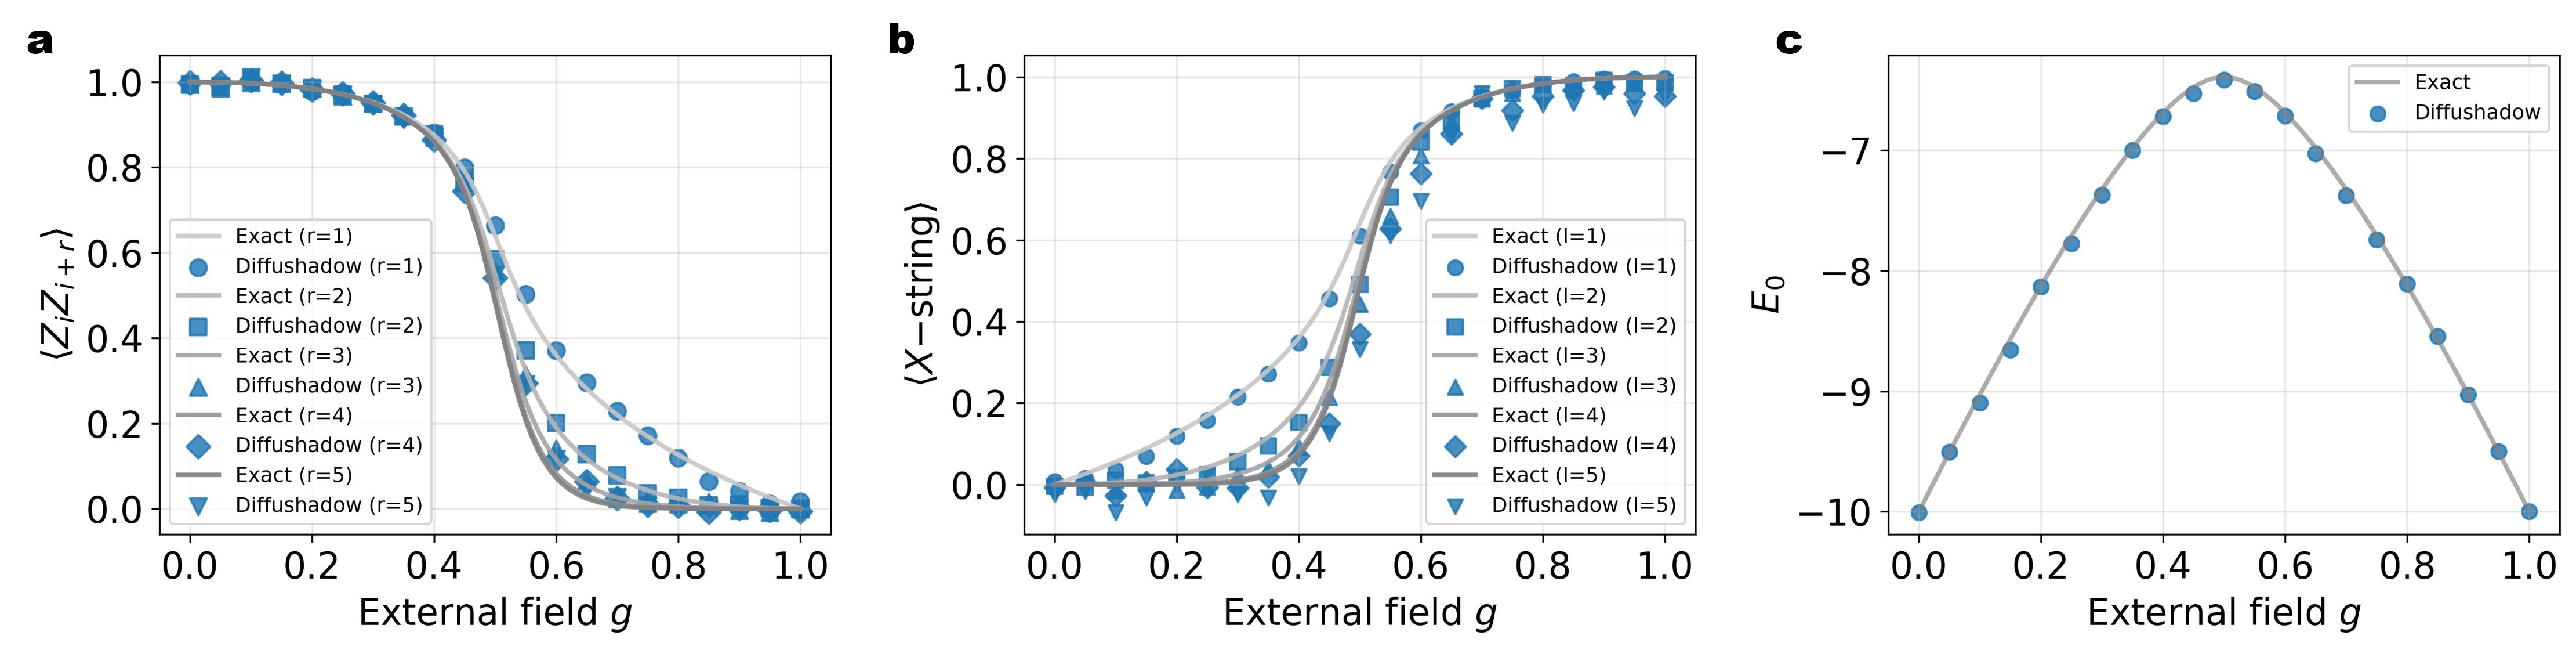
\includegraphics[width=\textwidth]{figures/Figure_10q_all.png}
  \caption{Additional observable estimation in the transverse-field Ising model. 
Ground-state observables of the 10-qubit transverse-field Ising model estimated from Diffushadow-generated classical-shadow measurements. 
(a) Two-point spin correlations \(\langle Z_i Z_{i+r}\rangle\) for different correlation distances \(r\). 
(b) \(X\)-string order parameters with different string lengths \(\ell\). 
(c) Ground-state energy \(E_0\). 
Grey solid curves denote exact diagonalization results, and blue markers denote estimates obtained from Diffushadow-generated classical-shadow measurements. 
In panels a and b, marker shapes distinguish the correlation distance \(r\) and the string length \(\ell\), respectively. 
These additional observables complement the longitudinal spin-correlation results emphasized in the main text and show that Diffushadow-generated shadows support estimation of both local correlations, extended string observables and the ground-state energy.}
  \label{fig:TFI_10q_all}    
\end{figure}


\sechead{S6}{Additional finite-size observable validation}
\label{supp:additional_validation}

\subhead{TFI correlations, strings and energy}
Supplementary Fig.~\ref{fig:TFI_10q_all} tests observables beyond the representative TFI
correlations emphasized in the main text. At $N=10$, generated Pauli
records are used to estimate $ZZ$ correlations at $r=1,\ldots,5$,
$X$ strings of length $\ell=1,\ldots,5$, and the total energy $E_0$.
The operators, spatial averages and MoM order are defined in Section~\ref{supp:shadow_estimators}.
The evaluation uses 15 uniformly spaced values of $g\in[0,1]$ and
$M=10{,}000$ records at each value. 
% \TBD{TFI-VALIDATION-CKPT: identify the checkpoint and generation seeds used for Supplementary Fig.~1}.

The generated-data estimates follow the ED reference trends: longitudinal
correlations decrease as the transverse field grows, while the displayed
$X$-string expectations increase. The energy also follows the reference
curve. This comparison supports agreement for the selected local,
extended-string and Hamiltonian observables at the tested size. It does
not establish equality of the complete measurement distributions.
The decoding comparisons for the string observables are discussed in
Section~\ref{supp:decoding_budget} rather than repeated here.




% \subhead{$J_1$--$J_2$ and ANNNI validation at $N=12$ and $N=24$}
% We further validate finite-size observables at $N=12$, which belongs
% to the initial training-size set, and $N=24$, which lies outside
% that set (Supplementary Fig.~\ref{fig:J1J2_ANNNI_12_24}).
% For the $J_1$--$J_2$ chain with $J_1=1$, we compare spin-dot
% correlations at $r=1,2$ across $J_2$. For the ANNNI chain at
% $\kappa=0.4$, we compare $S_{Z,N}(\pi)$ and $S_{Z,N}(\pi/2)$
% across $g$, using the normalization in
% Eq.~\eqref{supp:eq:annni_sf}. In both cases, observable estimates
% from Diffushadow-generated classical-shadow measurements are
% compared with finite-size exact-diagonalization references.
% \TBD{FRUSTRATED-VALIDATION: identify the
% first-round checkpoints, parameter grids, record counts, seeds and
% finite-size reference files}. The results are to be collected in
% \TBD{FIG-FRUSTRATED: Supplementary figure number and completed panels}.

% \TBD{FRUSTRATED-RESULTS: insert the verified comparison of the $N=12$
% and $N=24$ estimates with ED, and any numerical error statistic actually
% computed}. These checks evaluate transfer to the stated finite size;
% the thermodynamic-limit fits and the recursive-round comparison are
% reported separately in Section~S5 and Section~S10.


% \begin{figure}[htbp]
%   \centering
%   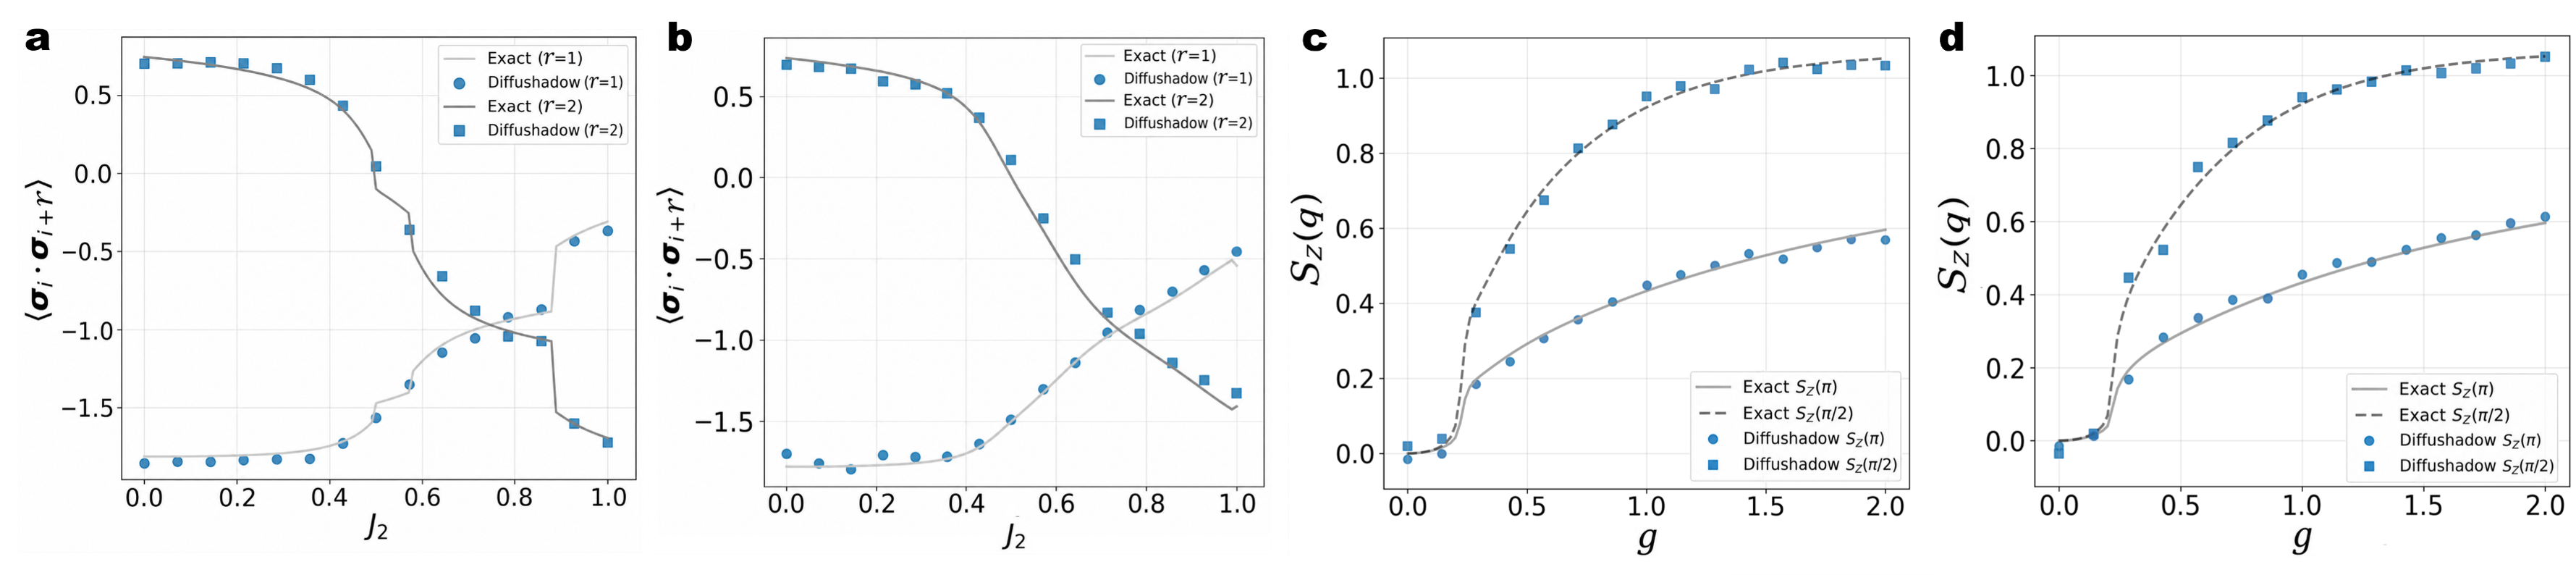
\includegraphics[width=\textwidth]{figures/Figure_J1J2_ANNNI_12_24.png}
%   \caption{\textbf{Finite-size observable validation for the
% $J_1$--$J_2$ and ANNNI chains.}
% \textbf{a,b,} Spin correlations
% $\langle\boldsymbol{\sigma}_i\cdot
% \boldsymbol{\sigma}_{i+r}\rangle$ at separations $r=1$ (circles)
% and $r=2$ (squares) for the $J_1$--$J_2$ model with $J_1=1$,
% shown as functions of $J_2$ for $N=12$ (\textbf{a}) and
% $N=24$ (\textbf{b}).
% \textbf{c,d,} Longitudinal structure factors $S_Z(q)$ at
% $q=\pi$ (circles) and $q=\pi/2$ (squares) for the ANNNI model
% at fixed $\kappa=0.4$, shown as functions of $g$ for
% $N=12$ (\textbf{c}) and $N=24$ (\textbf{d}).
% Blue markers denote estimates from Diffushadow-generated
% classical-shadow measurements, and grey lines denote exact
% finite-size references. The two sizes represent a system size
% included in the initial training data and a larger size absent
% from those data, respectively.}
%   \label{fig:J1J2_ANNNI_12_24}    
% \end{figure}


\sechead{S7}{Dependence on decoding strategy and sampling budget}
\label{supp:decoding_budget}

\subhead{Decoding strategy and number of updates}
We compare decoding protocols on the $N=10$ TFI benchmark using the
observable definitions in Section~\ref{supp:shadow_estimators}. Entropy-based decoding selects
the remaining site or sites with the lowest predictive entropy;
random-position decoding chooses among the remaining sites uniformly.
One-shot decoding fills all outcomes from a single model evaluation of
the fully masked sequence. The position-selection rule and the
outcome-value rule are distinct settings. 
% \TBD{ABLATION-VALUE-RULE:
% confirm probability sampling or argmax, temperature and random seeds
% for each existing comparison}. The full executable protocols, including
% the ShadowGPT training and generation settings, belong in Section~S3.

Supplementary Fig.~\ref{fig:diffusion_steps} compares $T=1,2,5,10$ updates. At $N=10$, these
settings reveal $10,5,2,1$ sites per update, respectively, with
predictions recomputed after each group of sites has been filled.
% \TBD{STEP-RUNS: checkpoint, per-parameter record count, parameter grid,
% generation seeds and confirmation that revealed tokens remain fixed
% in each retained run}. 
The curves show the strongest
one-shot deviations in the low-field correlation and energy estimates.
More updates improve agreement for these observables by making newly
generated outcomes available to later predictions. The improvement from additional denoising steps is especially visible in the low-field regime \(g < 0.5\), where the transverse-field Ising ground state exhibits stronger longitudinal order and longer-range spin correlations. In this regime, accurately generating globally consistent measurement outcomes requires the model to capture correlations across multiple sites, and gradual denoising provides a useful mechanism for progressively establishing these correlations. By contrast, in the high-field paramagnetic regime \(g > 0.5\), longitudinal correlations become weaker and more short-ranged, making the generated observables less sensitive to the number of refinement steps.

Supplementary Table~\ref{tab:mse_table} compares ShadowGPT, random-position
decoding, one-shot decoding and entropy-based iterative decoding at
$g=0.1,0.5,0.9$. Diffu-rdm denotes iterative decoding with randomly selected positions, Diffu-s1 denotes one-step decoding, and Diffu denotes the full entropy-based iterative decoding strategy. The one-step variant shows substantially larger errors, especially for the ground-state energy, confirming the importance of iterative denoising. Random position selection can perform competitively for some individual observables, but is less consistent than the full entropy-based strategy. Overall, full Diffushadow achieves low errors across representative observables and provides a stable alternative to sequential autoregressive generation.

\begin{figure}[htbp]
  \centering
  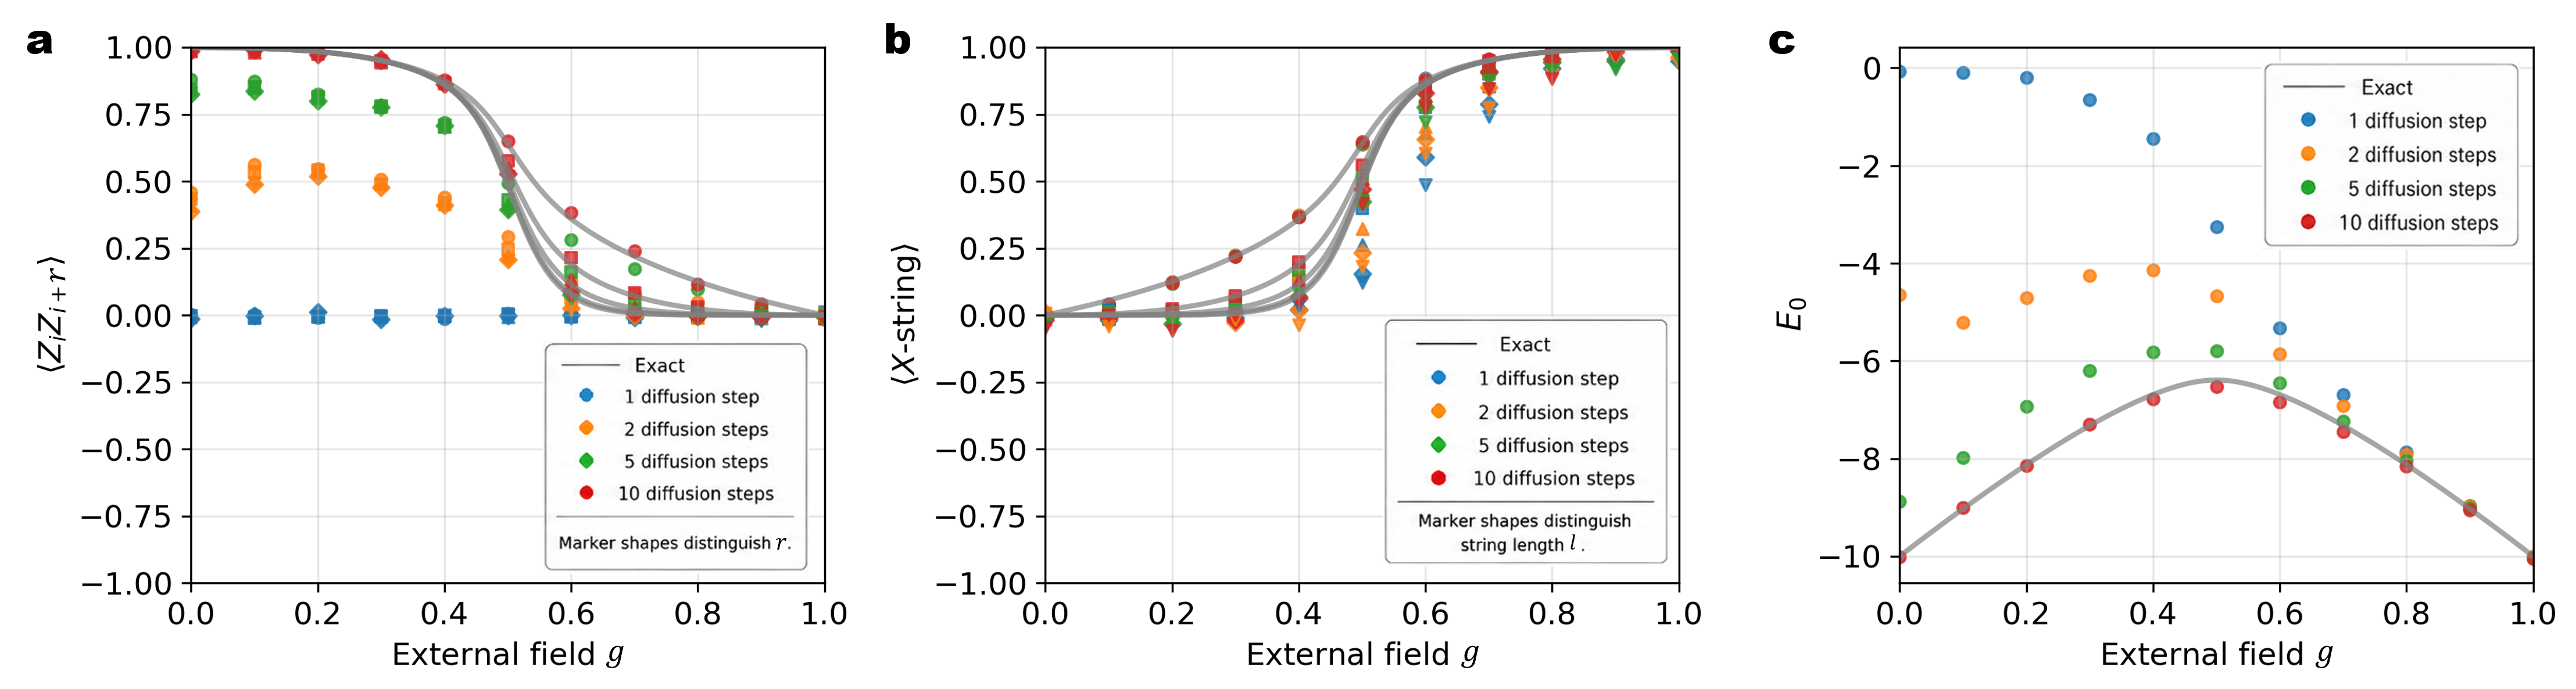
\includegraphics[width=\textwidth]{figures/Figure_diffusion_steps1.2.png}
  \caption{Effect of denoising steps on observable estimation in the transverse-field Ising model. 
Physical observables of the 10-qubit transverse-field Ising model estimated from Diffushadow-generated classical-shadow measurements using different numbers of denoising steps. 
(a) Two-point spin correlations \(\langle Z_i Z_{i+r}\rangle\). 
(b) \(X\)-string order parameters with different string lengths \(\ell\). 
(c) Ground-state energy per site \(E_0/N\). 
Grey solid curves denote exact diagonalization results, and colored markers denote Diffushadow estimates generated with 1, 2, 5 and 10 denoising steps. 
In panel a, marker shapes distinguish the correlation distance \(r\); in panel b, marker shapes distinguish the string length \(\ell\). 
Increasing the number of denoising steps improves the agreement between generated-measurement estimates and exact results, with one-step decoding showing the largest deviation and 10-step denoising giving the most accurate estimates.}
  \label{fig:diffusion_steps}    
\end{figure}


\begin{table}[htbp]
\centering
\small
\caption{MSE of selected observable estimates for the 10-qubit transverse-field Ising model. The table reports the ground-state energy \(E_0\) and representative \(X\)-string observables; \(ZZ\) correlations are omitted to avoid redundancy with the main text. ShGPT denotes ShadowGPT, Diffu-rdm denotes Diffushadow with randomly selected decoding positions, Diffu-s1 denotes one-step Diffushadow decoding, and Diffu denotes the full Diffushadow with entropy-based iterative decoding.}
\label{tab:mse_table}
\begin{tabular}{llcccc}
\hline
 &Model & $E_0$ & $\left(\prod_{i=1}^1 X_i\right)$ & $\left(\prod_{i=1}^3 X_i\right)$ & $\left(\prod_{i=1}^5 X_i\right)$\\
\hline
\multirow{4}{*}{$g=0.1$} 
& ShadowGPT      & $3.63{\times}10^{-4}$ & $7.56{\times}10^{-4}$ & $6.80{\times}10^{-4}$ & $2.77{\times}10^{-3}$\\
& Diffu-rdm & $2.34{\times}10^{-3}$ & $2.90{\times}10^{-4}$ & $1.88{\times}10^{-6}$ & $3.69{\times}10^{-3}$\\
& Diffu-s1  & $7.99{\times}10^{1}$ & $1.92{\times}10^{-4}$ & $1.16{\times}10^{-4}$ & $\underline{\mathbf{4.10{\times}10^{-4}}}$\\
& \textbf{Diffushadow}    & $\underline{\mathbf{2.77{\times}10^{-4}}}$ & $\underline{\mathbf{2.20{\times}10^{-4}}}$ & $\underline{\mathbf{1.85{\times}10^{-7}}}$ & $1.33{\times}10^{-3}$\\
\hline
\multirow{4}{*}{$g=0.5$} 
& ShadowGPT      & $1.35{\times}10^{-2}$ & $6.31{\times}10^{-5}$ & $2.15{\times}10^{-4}$ & $2.77{\times}10^{-4}$\\
& Diffu-rdm & $7.59{\times}10^{-3}$ & $2.17{\times}10^{-4}$ & $6.00{\times}10^{-4}$ & $1.12{\times}10^{-2}$\\
& Diffu-s1  & $1.00{\times}10^{1}$ & $1.05{\times}10^{-4}$ & $5.82{\times}10^{-2}$ & $1.71{\times}10^{-1}$\\
& \textbf{Diffushadow}    & $\underline{\mathbf{7.13{\times}10^{-3}}}$ & $\underline{\mathbf{4.01{\times}10^{-5}}}$ & $\underline{\mathbf{4.90{\times}10^{-5}}}$ & $\underline{\mathbf{2.29{\times}10^{-4}}}$\\
\hline
\multirow{4}{*}{$g=0.9$} 
& ShadowGPT      & $6.79{\times}10^{-4}$ & $9.88{\times}10^{-6}$ & $4.76{\times}10^{-5}$ & $\underline{\mathbf{7.57{\times}10^{-5}}}$\\
& Diffu-rdm & $5.05{\times}10^{-4}$ & $6.57{\times}10^{-8}$ & $6.20{\times}10^{-4}$ & $4.28{\times}10^{-3}$\\
& Diffu-s1  & $1.47{\times}10^{-3}$ & $4.44{\times}10^{-6}$ & $4.33{\times}10^{-4}$ & $1.21{\times}10^{-3}$\\
& \textbf{Diffushadow}    & $\underline{\mathbf{4.98{\times}10^{-4}}}$ & $\underline{\mathbf{3.32{\times}10^{-6}}}$ & $\underline{\mathbf{2.22{\times}10^{-8}}}$ & $3.88{\times}10^{-4}$\\
\hline
\end{tabular}
\end{table}


\subhead{Number of generated records}
Supplementary Fig.~\ref{fig:sample_size} compares $M=8000$, $10{,}000$, $100{,}000$ and
$300{,}000$ generated records per parameter point at $N=10$. Each
ensemble is processed with $K=10$ groups; the resulting group sizes
are $800$, $1000$, $10{,}000$ and $30{,}000$ records. The same $ZZ$
correlations, $X$ strings and total-energy observables are used.
% \TBD{BUDGET-RUNS: confirm checkpoint, decoding settings, parameter grid,
% seeds and whether the budgets are nested subsets or independently
% generated ensembles}.
The displayed observable trends are already recovered at the smaller
budgets and remain similar over the tested range. Larger ensembles
produce smoother curves in these plots. However, even the smaller sampling budgets already recover the main observable trends, including the decay of longitudinal spin correlations, the growth of \(X\)-string observables and the ground-state energy curve. These results suggest that the agreement with exact results is not solely a consequence of using an extremely large number of generated samples, but also reflects the quality of the measurement distribution learned by Diffushadow.

\begin{figure}[htbp]
  \centering
  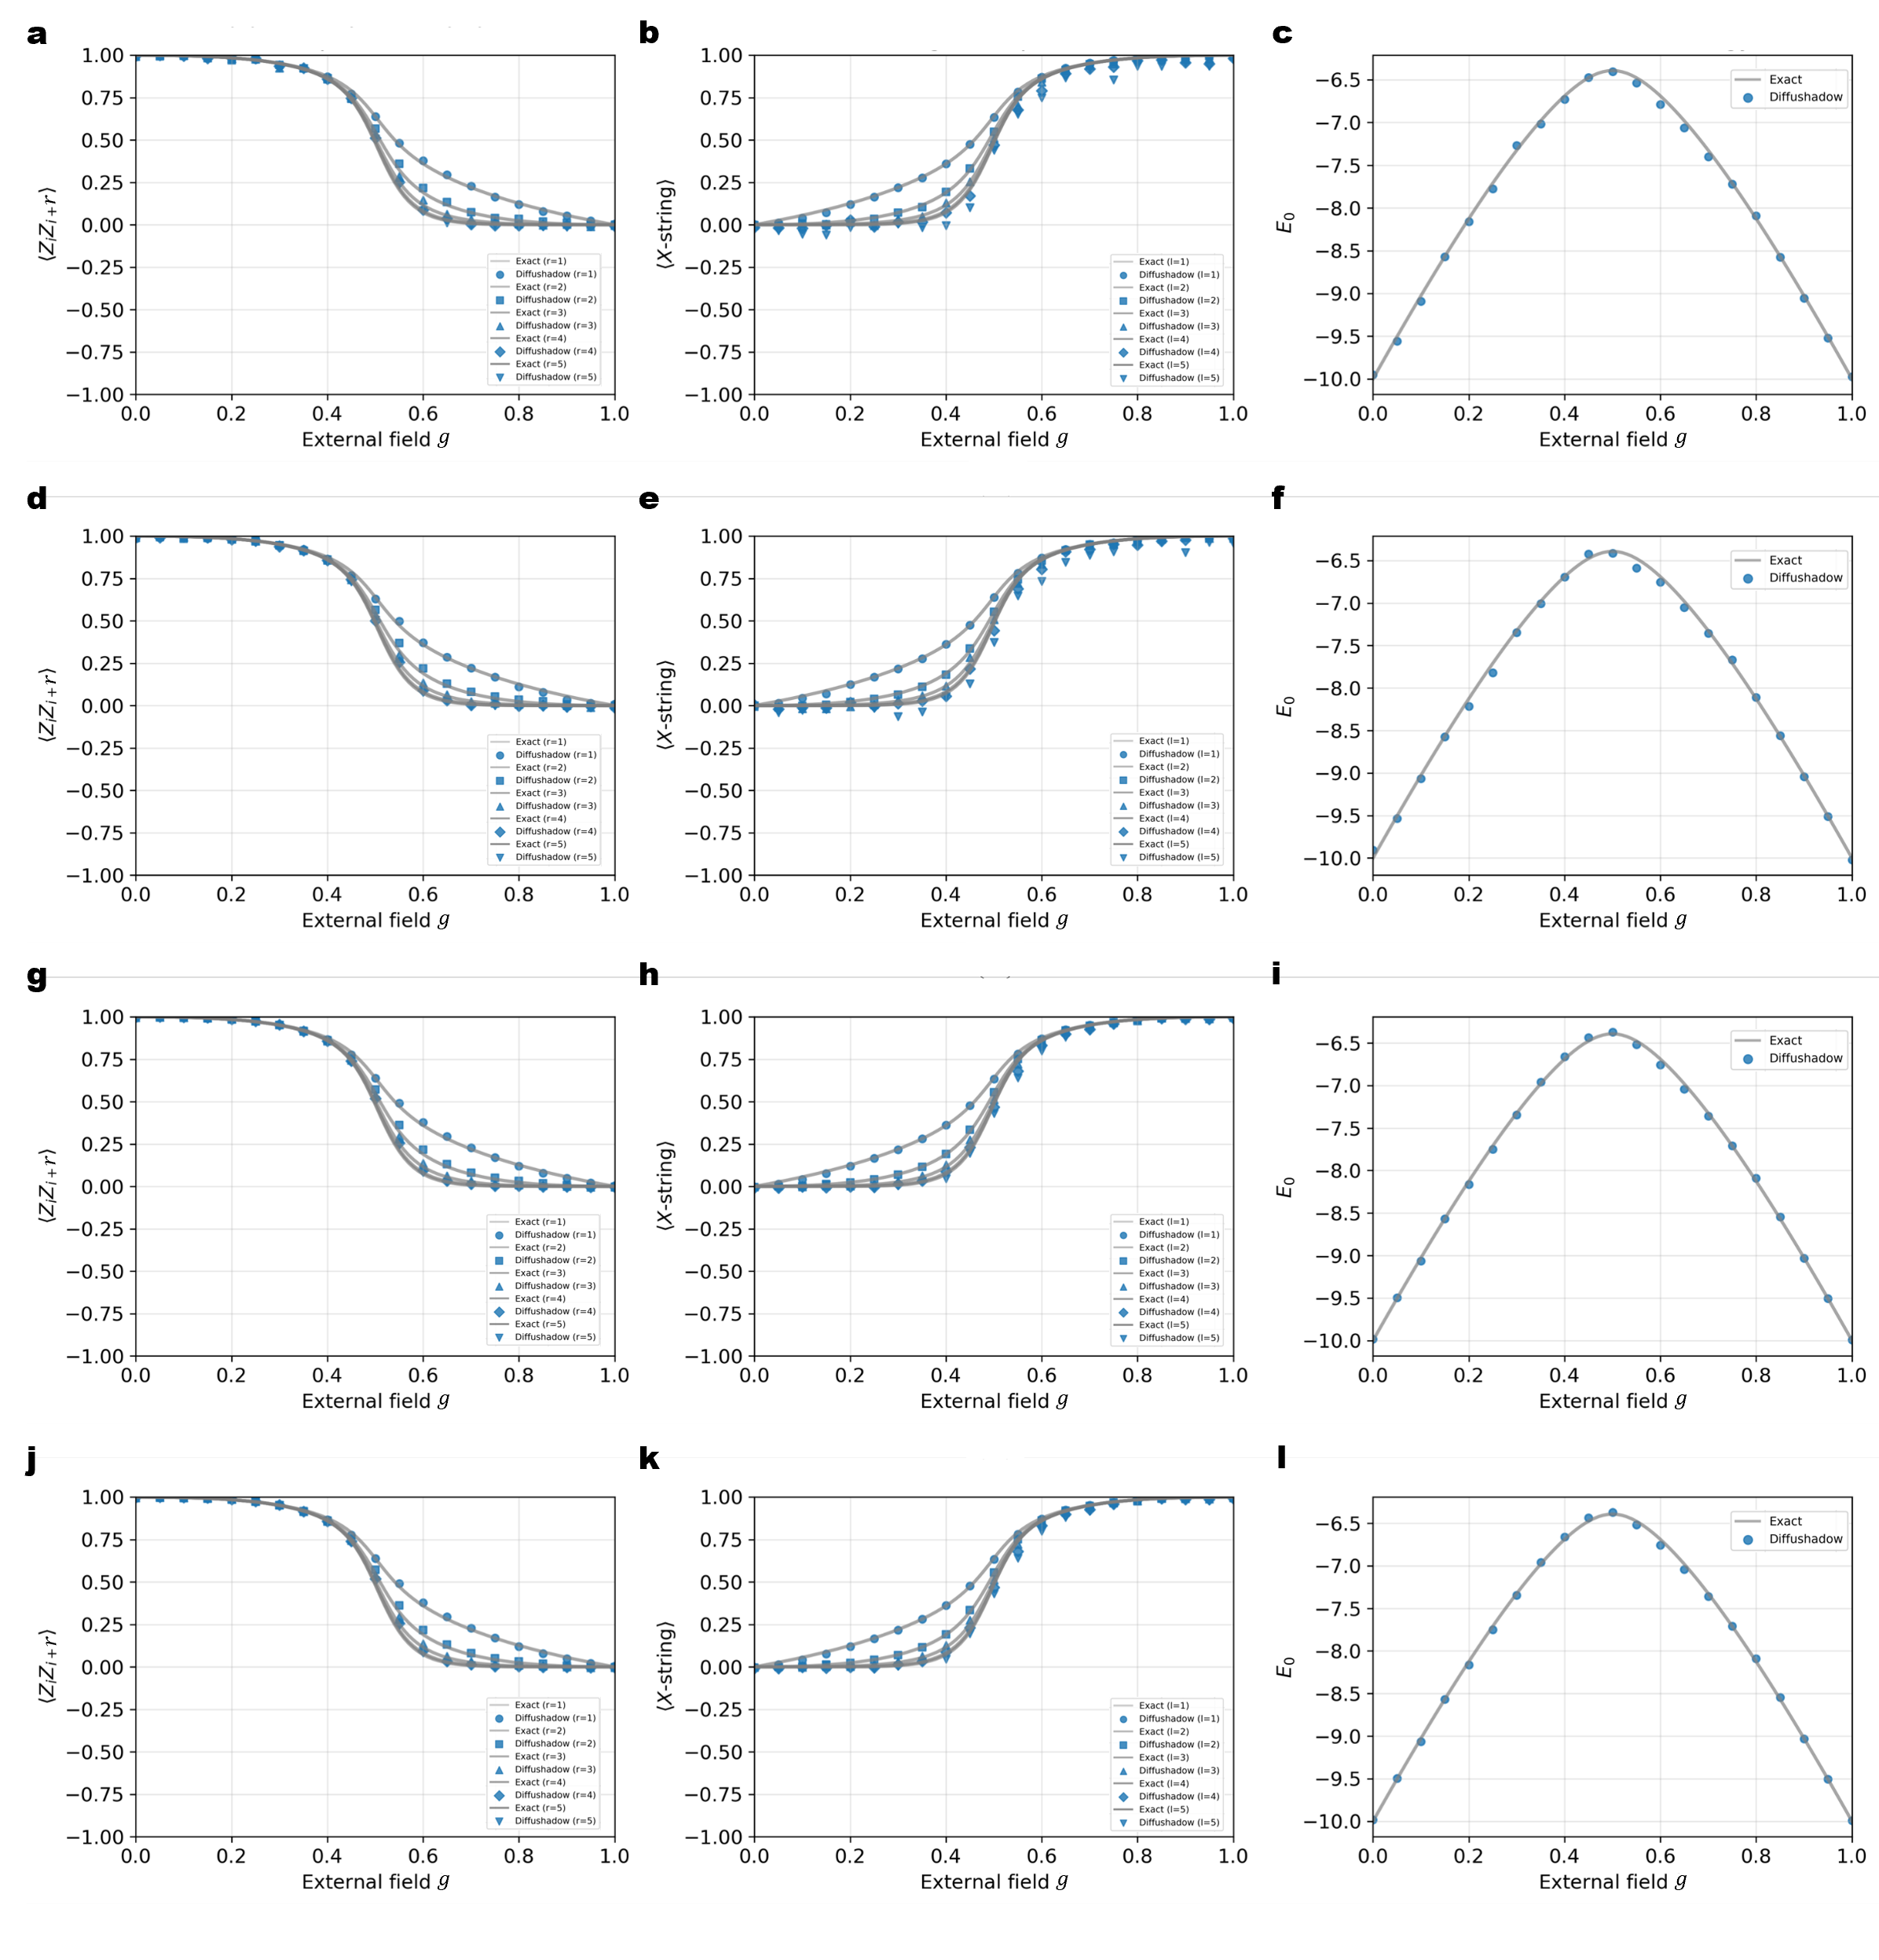
\includegraphics[width=\textwidth]{figures/Figure_sample_size1.4.png}
  \caption{Dependence of observable estimation on the number of generated classical-shadow snapshots in the transverse-field Ising model. 
Ground-state properties of the 10-qubit transverse-field Ising model estimated from Diffushadow-generated classical-shadow measurements using different numbers of generated snapshots \(M\). 
Panels a--c, d--f, g--i and j--l correspond to \(M=8\mathrm{k}\), \(10\mathrm{k}\), \(100\mathrm{k}\) and \(300\mathrm{k}\), respectively. 
In each row, the left panel shows the two-point spin correlations \(\langle Z_i Z_{i+r}\rangle\), the middle panel shows the \(X\)-string order parameters \(\langle X\text{-string}\rangle\) with different string lengths, and the right panel shows the ground-state energy per site \(E_0/N\). 
Grey solid curves denote exact diagonalization results, and blue markers denote estimates obtained from Diffushadow-generated measurements. 
In the correlation and string-order panels, different marker shapes distinguish different correlation distances \(r\) and string lengths \(l\), respectively. 
As the number of generated snapshots increases, the estimated observables remain consistently close to the exact results, indicating that Diffushadow provides stable physical-property estimation across different sampling budgets.}
  \label{fig:sample_size}    
\end{figure}


% \sechead{S8}{Consistency across recursive rounds}
% \label{supp:recursive_calibration}

% % \subhead{Fixed-size comparison across rounds}
% Supplementary Fig.~\ref{fig:stability_analysis} evaluates the first-, second- and third-round
% models at the common size $N=24$. Every round is initialized and
% trained from scratch. Round 1 uses exact records at $N=8,10,12,14$;
% round 2 retains exact $N=12,14$ records and adds round-1 records at
% $N=18,20,22,24$; round 3 retains exact $N=12,14$ records and adds
% round-2 records at $N=24,32,40,48$. 
% % The complete per-Hamiltonian
% % dataset and checkpoint manifest is provided in Section~S5.

% At $N=24$, the comparison includes TFI $ZZ$ correlations at $r=1,2,3$,
% $J_1$--$J_2$ spin-dot correlations at $r=1,2,3$, and ANNNI structure
% factors at $q=\pi,\pi/2$. 
% % \TBD{ROUND-COMPARISON-RUNS: verify the three
% % checkpoints for each Hamiltonian, evaluation grids, generated record
% % counts, seeds and the numerical reference shown in each panel}.
% The curves show similar estimates across the three rounds
% for these observables. This fixed-size check provides no indication of
% large drift in the displayed statistics at $N=24$. These results suggest that the recursive scale-extrapolation procedure is stable at the tested target size. In particular, adding generated measurements in later rounds does not substantially degrade the physical observables estimated from newly generated classical-shadow data.

% \begin{figure}[htbp]
%   \centering
%   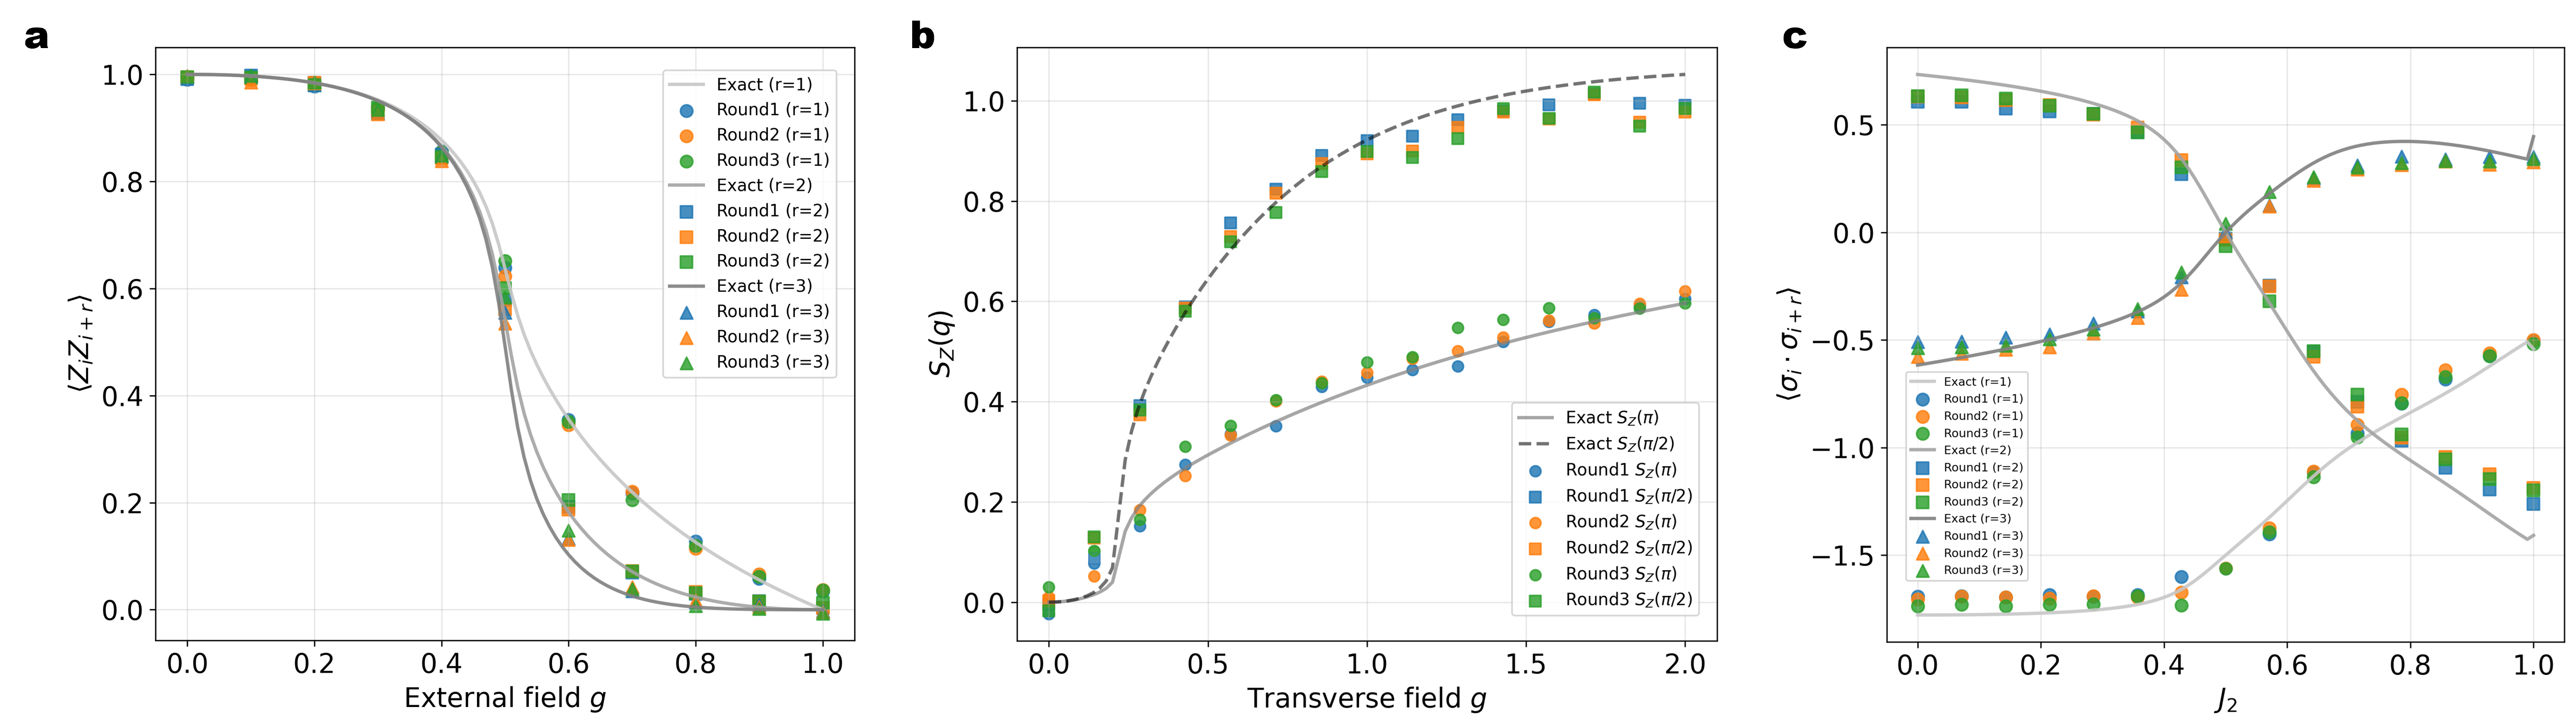
\includegraphics[width=\textwidth]{figures/Figure_stability_all2.0.png}
%   \caption{Stability of recursive scale extrapolation across training rounds.
% Comparison of observable estimates generated by Diffushadow models obtained from different recursive training rounds, evaluated at the same 24-qubit target system size.
% (a) Transverse-field Ising spin-spin correlations \(\langle Z_i Z_{i+r}\rangle\) for \(r=1,2,3\).
% (b) ANNNI structure factors \(S_Z(\pi)\) and \(S_Z(\pi/2)\).
% (c) $J_1$--$J_2$ spin-dot correlations \(\langle \boldsymbol{\sigma}_i\cdot\boldsymbol{\sigma}_{i+r}\rangle\) for \(r=1,2,3\).
% Solid or dashed curves denote exact diagonalization results, while markers denote observables estimated from Diffushadow-generated classical-shadow measurements.
% The close agreement among the three recursive rounds indicates that recursive scale extrapolation does not introduce substantial drift in the generated measurement distributions at the tested system size.}
%   \label{fig:stability_analysis}    
% \end{figure}

% \subhead{Calibration of the finite-size extrapolation form}
% Extended Data Fig.~2 compares linear and quadratic extrapolation of
% numerical finite-size TFI reference correlations. For each $g$ and
% distance $r$, the two forms are
% \begin{equation}
% O_N=O_\infty+\frac{a}{N},\qquad
% O_N=O_\infty+\frac{a}{N}+\frac{b}{N^2}.
% \label{supp:eq:calibration_fits}
% \end{equation}
% The main-text generated-data analysis uses the linear form. The
% quadratic form is a calibration comparison, not an additional term
% implicitly included in the reported main-text fits.

% The final TFI generated-data fit sets are
% $\{10,12,16,18,20,22,24,32,36,48,64,72,96\}$ for $r=1$ and
% $\{24,32,36,48,64,72,96\}$ for $r=10$.
% \TBD{CALIBRATION-INPUTS: identify the numerical finite-size reference
% method and files, verify the actual sizes and parameter grid used in
% Extended Data Fig.~2, and match its infinite-system reference}.
% \TBD{CALIBRATION-RESULT: insert the verified comparison of the fitted
% intercepts with the reference, without inferring a quantitative bound
% from the plot alone}. This calibration separates finite-size fit error
% on numerical reference data from error arising in generated records.
% Its conclusions apply to the tested observables, parameter range and
% size window; they do not establish a universal $1/N$ expansion.

% Sampling intervals for generated-data estimates are obtained from
% $B=1000$ bootstrap replicates of whole records, recomputing $K=10$
% MoM estimates and refitting at each replicate, as detailed in Section~S5.
% The 2.5th and 97.5th percentiles give pointwise 95\% intervals.
% The generator and the chosen fit form remain fixed. These intervals
% propagate finite-record sampling uncertainty and do not include
% generation bias, inherited recursive error or uncertainty in choosing
% between the linear and quadratic forms.

\sechead{S8}{Additional Rydberg reconstruction diagnostics}
\label{supp:rydberg_results}

These diagnostics supplement the occupation structure factor and
missing-site accuracy in Fig.~4. They use $N=32$, $R_b/a=2.35$,
$f=0.3$ and $k=10$ uniformly chosen missing sites per record.
The intact, conditional-sampling and unconditioned-fill ensembles
share the same $M_d=1000$ records and masks at each of the four original
detunings. The definitions and comparison protocol are given in
Section~\ref{supp:rydberg}. Conditional ensemble results use probability sampling at
$\tau=1$, rather than the argmax completion used for site accuracy.

\subhead{Consistency across observed and reconstructed neighbours}
We evaluate nearest-neighbour double excitations across the boundary
between observed and reconstructed sites. For each detuning, 10 sites
are randomly masked in each of 1000 held-out records at $N=32$.
A neighbouring pair is included when exactly one of its sites is
masked, giving approximately $1.38\times10^4$ scored pairs per
detuning. The same pair sets are used for intact records, conditional
completion and unconditioned fill (control). Counts and rates,
computed using Eq.~\eqref{supp:eq:blockade}, are listed below.
\begin{center}
\small
\begin{tabular}{@{}r r r r r r@{}}
\toprule
$d$ & Intact count & Conditional count & Conditional rate
& Control count & Control rate\\
\midrule
0.2 & 0 & 1 & $0.007\%$ & 225 & $1.63\%$\\
1.8 & 0 & 0 & $0.000\%$ & 312 & $2.26\%$\\
3.4 & 0 & 1 & $0.007\%$ & 15 & $0.11\%$\\
5.0 & 0 & 2 & $0.014\%$ & 508 & $3.68\%$\\
\bottomrule
\end{tabular}
\end{center}
Across the four detunings, conditional completion produces four
doubly excited boundary pairs, compared with 1060 for unconditioned
fill. The conditional rates remain below $0.02\%$ at every detuning.
These results support the role of conditioning on the observed
occupations in preserving blockade consistency across the
reconstruction boundary.

\subhead{Multisite observables and complete-case sample counts}
At $d=5.0$, we evaluate the period-three products $G_\ell$ at
$\ell=2$ and $\ell=8$ to assess whether conditional completion
preserves multisite statistics. The estimates from intact records,
conditional completion and unconditioned fill (control), together
with the mean numbers of records available to the complete-case
estimator, are listed below.
\begin{center}
\begin{tabular}{@{}r r r r r@{}}
\toprule
$\ell$ & Intact $G_\ell$ & Conditional $G_\ell$ & Control $G_\ell$
& Mean usable records\\
\midrule
2 & 0.297 & 0.295 & 0.271 & 467\\
8 & 0.064 & 0.062 & 0.026 & 28\\
\bottomrule
\end{tabular}
\end{center}
The complete-case counts are averaged over spatial origins, as
defined in Eq.~\eqref{supp:eq:usable}, out of 1000 held-out records.
A record contributes at a given origin only when all sites involved
in the product are observed. Conditional completion uses all 1000
records at every valid origin.

For both orders, the conditional estimates closely reproduce the
intact values, whereas unconditioned fill gives lower estimates.
The reduction in complete-case counts from 467 at $\ell=2$ to
28 at $\ell=8$ illustrates the loss of usable records for higher-order
observables. Conditional completion retains the full ensemble
for estimating both products.

\subhead{Excitation-number fluctuations}
For each record $s$, we define the total excitation number as
$Q_s=\sum_i n_i^{(s)}$. At $d=5.0$, the mean excitation numbers
are 10.72 for intact records and 10.68 for conditional completion.
The population standard deviations across records are 0.521,
0.538 and 1.168 for intact records, conditional completion and
unconditioned fill, respectively. Conditional completion closely
reproduces both the mean and the fluctuations of the intact ensemble,
whereas unconditioned fill produces substantially larger
excitation-number fluctuations.

\bibliographystyle{unsrtnat}
\phantomsection
\addcontentsline{toc}{section}{References}
\bibliography{supplementary_refs}

\end{document}
